
%\textbf{中文摘要和中文关键词}

% 摘要内容应概括地反映出本论文的主要内容\footnote{这是另一个脚注},主要说明本论文的研究目的、内容、方法、成果和结论。语言力求精练、准确,摘要字数300字左右。


%\begin{enumerate}
%    \item 科学技术名词术语尽量采用全国自然科学名词审定委员会公布的规范词或国家标准、部标准中规定的名称,尚未统一规定或叫法有争议的名词术语,可采用惯用的名称。
%    \item 特定含义的名词术语或新名词、以及使用外文缩写代替某一名词术语时,首次出现时应在括号内注明其含义。
%    \item 外国人名一般采用英文原名,可不译成中文,英文人名按姓前名后的原则书写。一般很熟知的外国人名(如牛顿、爱因斯坦、达尔文、马克思等)可按通常标准译法写译名。
    
%\end{enumerate}


% \begin{itemize}
%     \item	封面(见附件)
% \item	学术声明(见附件)
% \item	中文摘要及关键词
% \item	外文摘要及关键词
% \item	标题及目录
% \item	正文
% \item	参考文献
% \item	附录(如果有)
% \item	致谢
% \item	封底(见附件)
% \end{itemize}
\section{绪论}
\subsection{选题背景及研究意义}
\subsubsection{选题背景}
2019年年底,新型冠状病毒席卷全球,是进入21世纪以来史上最大规模的冠状病毒流行病。时隔两年,在新型冠状病毒逐渐被抑制之后,其变异株奥密克戎迅速在全球范围内传播,具有更强的传染性和致病率。
自2021年起,奥密克戎变异株出的诞生,以超强的感染力在数百个国家间迅速传播。根据中国国家卫健委的数据,在2022年2月到5月,每日新增病例最高超过2万例\cite{zhang2022shanghai}。由于感染人数的无法控制,之前的防控策略受到冲击,对于如何平衡防治病毒与民生经济,是政府面临的最重要的问题\cite{张佳琦2022新型冠状病毒奥密克戎变异株的研究进展}。
奥密克戎变异株(BA.1.1.529)来自BA.1.1谱系,是新型冠状病毒的进化支系之一\cite{giovanetti2021evolution}。Chen\cite{chen2022omicron}等人计算得出奥密克戎变种的传播率比原始病毒强13倍。
张佳琦\cite{张佳琦2022新型冠状病毒奥密克戎变异株的研究进展}表明奥密克戎变异株多个基因位点的突变,增强了病毒复制能力和受体亲和力,进而提高了它的传染性和致病能力,并有一定可能影响抗体识别,导致疫苗失效。

Wu\cite{wu2022epidemiologic}等人通过SEIR模型比较了奥密克戎与Delta变异株的传染力,发现比Delta强约37.5\%。Bastard\cite{bastard2022impact}等人研究了奥密克戎变体的影响,发现人群感染力明显增加,感染间隔时间短,但感染的病例占比较低。
来自Menni\cite{menni2022symptom}等人的调查样本显示,接种疫苗后的感染奥密克戎群体最常出现的症状为:流涕(76.5\%)、头痛(74.4\%)、喉咙痛(70.5\%)、打喷嚏(63.5\%)、持续性咳嗽(49.8\%),与之相对的,重症病例减少、住院率较低。但是重症率的降低不能忽视它的危害,奥密克戎一个人平均可以感染十个人左右,Strasser\cite{strasser2022sars}等人表明奥密克戎只是因为政府更充分的应对措施及更好的治疗才导致重症率减少,但实际上致死率和早期新型冠状病毒一样严重。

奥密克戎变异株的防控干预措施与早期新冠病毒有所不同,应该采取更加高效、快捷的防控体系;由欧阳康\cite{欧阳康2022新冠肺炎病毒变异传播背景下的疫情精准防控体系研究}的文章可知,需要提升疫情监测能力,在疫情出现开始快速核酸检测,防止疑似病例进入人群密集地区,在一个潜伏期左右控制住疫情传播。个人卫生应注意佩戴好口罩,保持安全距离,在公共场合用酒精消毒,减少非必要外出等。
由Xu\cite{xu2022protective}等人可知在接种加强针疫苗后,预防效果显著,但会随着时间推进而减弱,许多新型冠状病毒疫苗对奥密克戎变体的效果不显著,给医药体系带来巨大压力。

综上,我们发现奥密克戎变异株通过传染性强、逃逸能力高等特点对这个社会群体造成巨大威胁,对应的疫苗研发进展缓慢,为了避免过高的感染率以及经济衰退,政府部门要协调人群流动,提出封控策略来稳定社会。

\subsubsection{研究意义}

作为人类历史上破坏性最强的流行病之一,从2019年底开始的COVID-19已经对世界各国造成了巨大的影响,如今奥密克戎变体的出现又再一次延续了群众的恐慌情绪。政府相关部门应采取创新有效的手段予以应对。Flaxman\cite{flaxman2020estimating}和Kucharski\cite{kucharski2020early}等人已经研究了很多防控方法来阻碍疾病的传播,例如,让政府加快核酸监测、药物疫苗研发等医疗措施;以及一些简单的个人防控如外出戴口罩并保持一定的社交距离。
但这些措施不能从根本上保证在未研发出疫苗的疫情前期,人群会完全理性地遵守研究机构提出的建议保证自己的防控规范,所以最有效的防控新冠病毒的方法是政府对社会群体的强制干预,即封控策略,在一定时间内停止人类的社交活动,从而减缓疾病的传播,为疫苗研发接种提供时间。但是,封控措施会在社会上引起巨大争议,因为政府强制暂停人群的社交行动损失了绝大数人的即时利益,对我们的社会和经济将造成巨大影响,政府需同时考虑经济效应、人群病亡率以及群众情绪来调整封控策略。
政府怎么样以及什么时候实行封控措施对于相关研究学者和政治家来说是一个巨大的难题。本文为了解决这个问题,结合了流行病和经济学的数学模型。

流行病学模型被广泛应用于预测疫情的进程。然而关于经济决策和感染率之间的互动不多,比如封控策略如何影响人群的经济水平和疾病传播。Ferguson\cite{ferguson2006strategies}和Neil M\cite{ferguson2020report}等人使用带外生参数的流行病模型对政府风控进行分析,并通过数据模拟出的结果评价现实结果。在本文,我们扩展了修正SEIR模型,以研究经济决策和流行病动态之间的平衡相互作用。我们的模型具有流行病和经济之间的双向相互作用。以总死亡人数来衡量,人们决定减少消费和工作,从而降低了疫情的严重性,进而减缓了疫情造成的经济衰退。


\subsubsection{主要创新点}
本文在Eichenbaum\cite{eichenbaum2021macroeconomics}SIR模型的基础上针对COVID-19病毒奥密克戎变体,改进为修正后的SEIR模型来演进人群的变化过程,引入潜伏者这一人群来体现奥密克戎病毒的高传播性、高隐匿性,同时,针对奥密克戎变体虽然致死率下降但是恢复后抗体减弱的状况,我们引入复阳系数保证人群迭代的准确性。并且针对感染者和潜伏者我们采取了不同的遏制系数表明潜伏者在被检测出阳性前的不确定性。

不同于其他政府单独制定封控政策,本文专注于各类人群对奥密克戎和政府管控政策的考量,将人群的消费和工作时间等经济决策嵌入到简单的古诺均衡中并通过扩展到SEIR模型模拟人群相互之间的反应。与Eichenbaum\cite{eichenbaum2021macroeconomics}等人通过控制税率来制定最优遏制策略不同,本文设封控水平为控制系数,更加简单高效。

在本文中我们也引入一个死亡惩罚系数来调节封控策略的导向,从全局出发,使得求出的结论更具有普遍性,做出的预测人群和消费量变化更接近重视人民健康和幸福的国家。
\subsection{国内外研究综述}
\subsubsection{国内研究综述}
截至到现在,国内外许多专家学者使用不同的研究方法和模型对COVID-19病毒及其变种进行分析。

对于传染病模型的改进,张儆轩\cite{张儆轩2021考虑死亡因素和不同时段接触数的}等人考虑了带有死亡因素和不同时间接触数的SEIR模型,运用相轨线分析平衡点的全局稳定性,常瑜洋\cite{常瑜洋2023基于}考虑了无症状感染者及潜伏者人群代入到SEIR模型当中,同时通过第二代再生矩阵进行灵敏度分析;郭慧敏\cite{郭慧敏2023基于隔离人群的}考虑到奥密克戎的二次感染及“复阳”问题,建立具有隔离人群的SEIRS模型,由最小二乘法求得参数最优解;尹凌\cite{尹凌2021耦合人群移动的}从疫情短期预测和过程模拟两个角度,分类总结了耦合人群移动的COVID-19传染病模型。研究方法涵盖了人群移动一阶量与人群移动二阶量的耦合模型,以及群体级别和个体级别的耦合模型;李照\cite{李照2021一种耦合}基于地理信息系统(GIS)和长短时记忆网络(LSTM)算法,构建了一个模拟模型,用于研究传染病在空间和时间上的传播过程。
对于加入随机项的SIR模型,石佳欣\cite{石佳欣2022一类随机系统基本再生数的计算与应用}通过引入随机噪声,建立了具有随机扰动的SEIR模型;陈倩\cite{陈倩2023基于改进的随机}提出了改进的随机SEIR模型同时使用最小二乘法估计参数得出控制再生数;杨赟\cite{杨赟2022基于随机}基于2020年1月28日至2020年3月10日的湖北省疫情数据,考虑新型冠状病毒潜伏期的传播能力,建立了经典SEIR传播动力学模型和随机SEIR传播动力学模型。
针对SIR模型参数估计的方法,黄丽霞\cite{黄丽霞2023基于分阶段}建立了含有潜伏者及住院和无症状感染舱室的SEIR模型,同时自适应混沌粒子群算法进行参数估计;王建伟\cite{王建伟2020基于广义}应用SEIR模型估计参数,然后基于Anylogic仿真进行敏感性分析;宋倩倩\cite{宋倩倩2020新型冠状病毒肺炎的早期传染病流行病学参数估计研究}使用多种概率分布拟合从报告病历信息中获取的潜伏期和间隔数据,采用Akaike信息准则确定最优模型,利用指数增长法、最大似然法和SEIR模型估计基本再生数。
对于SIR模型的求解方法,程哲阳\cite{1021167897.nh}在疫情初期考虑了无症状感染者的存在,建立了SEIAQR模型,通过粒子群算法和搜索算法求解模型,计算基本再生数;燕杨\cite{燕杨2021基于改进}通过对传统SEIR模型进行优化,使其中的感染率参数带上衰减函数,对数据拟合得到随时间变化而变化的感染率,进而用ARIM算法对传播趋势进行预测。

\subsubsection{国外研究综述}
针对SIR模型的求解方法,Harko\cite{harko2014exact}等人以参数形式获得了SIR模型的精确解析解。同时把非线性微分方程组描述的SIR模型简化为阿贝尔方程,并用幂级数形式获得Abel的通解;Calvia\cite{calvia2024simple}等人运用HJB方法求解针对新冠疫情的最优隔离策略。
对于传染病模型的改进,McQuade\cite{mcquade2021control}等人追踪具体的干预措施,比如医院床位占用率以及对新泽西州不同区域的感染状况进行对比;Bohner\cite{bohner2019exact}等人研究了基于贝利连续微分系统的流行病模型。在连续时间上,将经典模型扩展到瞬态系数,并提出了Gleissner法的替代方法,并对SIR模型推导求解。
对于封锁策略的制定,Acemoglu\cite{acemoglu2021optimal}等人使用SIR模型进行有针对的封锁,发现针对风险/年龄组的最佳政策优于最佳统一政策,大部分收益可以通过采取更严格的保护措施来实现;Garriga\cite{garriga2022optimal}等人在动态模型中分析了流行病下的管理政策,包括居家和疫苗接种政策。其认为最佳管理政策是对就业大幅限制,然后在疫情高峰前部分放松,因此要以尽可能高的速度接种疫苗;Bairoliya\cite{bairoliya2023macroeconomic}等人认为不同群体的劳动生产率存在显著差异,其使用重叠世代模型模拟人群管控并与之前的封锁策略比较降低了疫情对经济造成的严重后果。

\subsection{研究内容}
本文扩展了SEIR模型来研究经济决策与流行病之间的均衡相互作用。在设定的SEIR宏观模型中人们工作时间和消费的减少会减轻疫情的严重程度,但会导致国家经济一定程度的衰退。在该模型中,最好的简单封控政策会加剧经济衰退的严重程度,但可以拯救更多人的生命。
同时我们所求的模型是理性的,会与现实中的人群感染数据存在差异,因为感染病毒的人不会完全理性做出利益最大化的决定,感染者的行为会对易感者的效用产生影响。\cite{garibaldi2020modelling}。

为了使得到的结果更加直观和易于理解,让人们能够更容易地理解结果的含义和推论,我们使用了一个相对简单的模型。它导致我们无法研究与疫情相关的许多重要政策问题。例如,我们不考虑减轻家庭和企业遭受的经济困难的政策,此类政策包括向家庭转移财政和贷款,以及一些政府的经济刺激计划或福利计划。

同时我们在文章的最也讨论了接种疫苗的情形,奥密克戎是强传播性的COVID-19变体,目前的疫苗研究已进入开发和生产阶段。许多国家正在进行大规模疫苗接种。从经济角度看,接种疫苗可能是恢复经济和社会正常的有效途径。封锁只能减缓流行病的传播,而接种疫苗则能防止人们感染疾病,从而使人们能够自由地工作和消费。

本文在获取各个参数的数据后,建立扩展SERI宏观模型,建立各类人群效用最大化的目标函数,通过对人群消费和工作时间的控制策略,转化为最优控制问题进行求解,最后对不同控制效果下的各类人群及其消费的时间走势图进行分析,为现实中的政策制定提供理论基础。全文分为四个章节。

第一章介绍了奥密克戎变体的传播特点、危害以及一些相关的防控措施,并分析了部分学者关于SIR基础传染病模型的研究。

第二章建立模型,首先建立带有潜伏者的SEIR模型,其次为了研究人群的福利水平,我们建立了效用模型来表达其获得的效用,并由于控制策略的原因对效用中的参数进行约束设定。

第三章为模型求解,首先通过KKT条件计算出每类人群的最大效用,然后通过给定控制水平将该问题转为最优控制问题进行求解。并通过使用公开数据进行参数估计得到计算最优效用的具体值,我们通过使用matlab工具箱fmincon函数中的内点法进行求解。
在求解模型中,我们分析了五种控制情况,分别为最优控制、带有死亡惩罚系数的最优控制、提前结束的最优控制、较晚开始的最优控制以及疫苗接种,对图中参数值进行比较分析,从而更好的评估现实中防控措施的实际效果。

第四章是对本文工作的总结和展望,并分析了一些奥密克戎病毒传播过程中可能面临的问题。
\autoref{fig:ima30}为本文的思维导图,为其提供了一个系统的框架。

\begin{figure}[htbp]
    \centering
    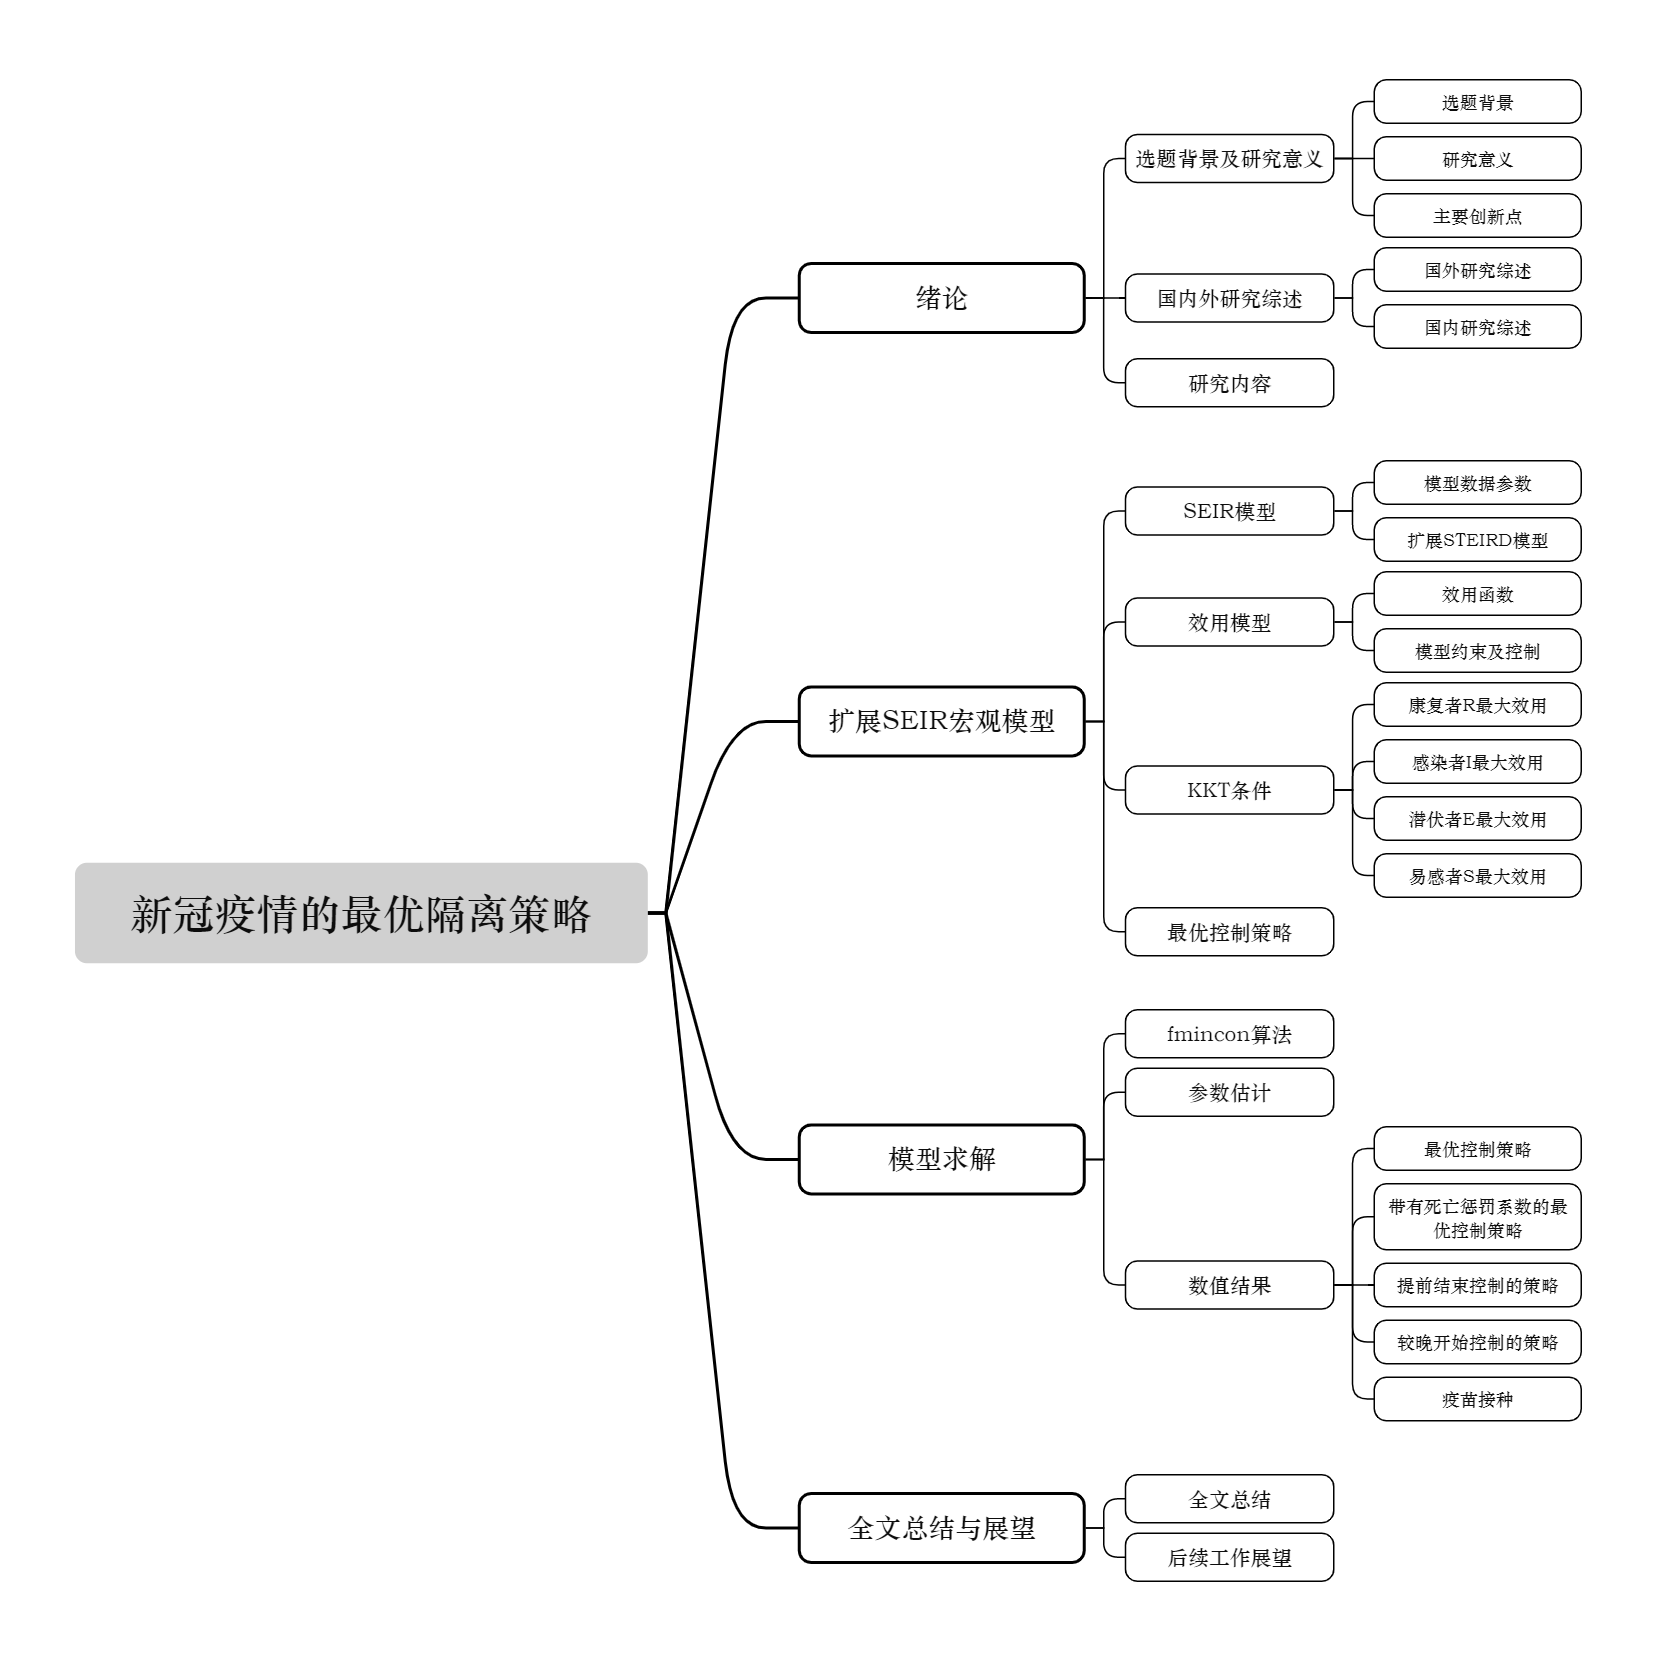
\includegraphics[width=1\textwidth]{fig/image059.png}
    \caption{思维导图}
    \label{fig:ima30}
\end{figure}
\vspace{110pt}
\section{扩展SEIR宏观模型}
\subsection{扩展SEIR模型}
\subsubsection{模型数据参数}
2021年11月全球受到奥密克戎的影响,新型冠状病毒感染(COVID-19)疫情进入新高峰。奥密克戎具有传染性强、传播速度快、隐匿性高、人群普遍易感等特点,给我国疫情防控带来了更大的压力和挑战。 

我们设$S_t$,$E_t$,$I_t$,$R_t$,$D_t$,$T_t$,$Pop_t$分别为t时刻的易感人群,潜伏人群,感染人群,康复人群,死亡人群,新增感染人群以及总人群,总人群在$t_0$时刻为$Pop_0=1$。

关于易感人群与携带病毒者的接触方式本文分为三种,分别为$\Pi_1$,$\Pi_2$和$\Pi_3$\cite{fu2022optimal},其中$\Pi_1$既表明人群在购物时间内被传染的情况,即人群消费购物越频繁,接触到携带病毒者的概率越大,也表示因该消费活动而感染的概率,$\Pi_2$表示为因工作接触而感染的概率,$\Pi_3$表示因为除了消费和工作之外其他原因导致感染的概率。

$\delta_v$为疫苗接种情况,在接种疫苗后,易感人群在下一个单位时间开始转入康复人群。假设在每个单位时间内研发出疫苗的概率为$\delta_v$,一旦研发出来,就立即向所有易感人群提供疫苗。
$\Pi_r$表示感染者以该概率康复,$\Pi_d$表示感染者以该概率死亡\cite{eichenbaum2021macroeconomics}。同时由于感染新冠的人群有部分人免疫力较低,且存在医护人员检测技术不到位等状况,进而体内有病毒残留导致出现“复阳”现象,据统计,我国的“复阳”病例占总体的比例较低,约在$5\%$至$15\%$之间,本文取$\xi=5\%$作为复阳概率\cite{郭慧敏2023基于隔离人群的}。
设$\sigma$为潜伏人群转化为感染人群的概率,其中$\frac{1}{\sigma}$为感染奥密克戎的潜伏期,由于奥密克戎的潜伏期一般为2\~{}3d,则本文设定该病毒被检测的时间为3d,$\sigma=\frac{1}{3}$\cite{杨利超2024基于真实世界数据的修正}。

\subsubsection{扩展STEIRD模型}
设$T_t$为在t时刻易感者(S)与潜伏者(E)和感染者(I)接触并感染的概率。本文中我们有三种接触方式,第一种为在购买消费情况下与感染者和潜伏者接触,这些互动导致的感染上的人数为$\Pi_1(S_t C_{t}^{s})(I_t C_{t}^{i}+E_t C_{t}^{e})$,其中$(S_t C_{t}^{s})$和$(I_t C_{t}^{i}+E_t C_{t}^{e})$分别表示易感者与潜伏者和感染者的消费支出;
第二种为在工作中互动导致的新的感染上的人数为$\Pi_2(S_t N_{t}^{s})(I_t N_{t}^{i}+E_t N_{t}^{e})$,其中$(S_t N_{t}^{s})$和$(I_t N_{t}^{i}+E_t N_{t}^{e})$分别表示易感者与潜伏者和感染者的工作时间;第三种为除了消费和工作这些行为的见面方式,例如,与邻居乘坐电梯、路上散步接触等,这些接触导致的感染人数为$\Pi_3 S_{t}(I_{t}+E_{t})$。
\vspace{32pt}
\begin{figure}[htbp]
    \centering
    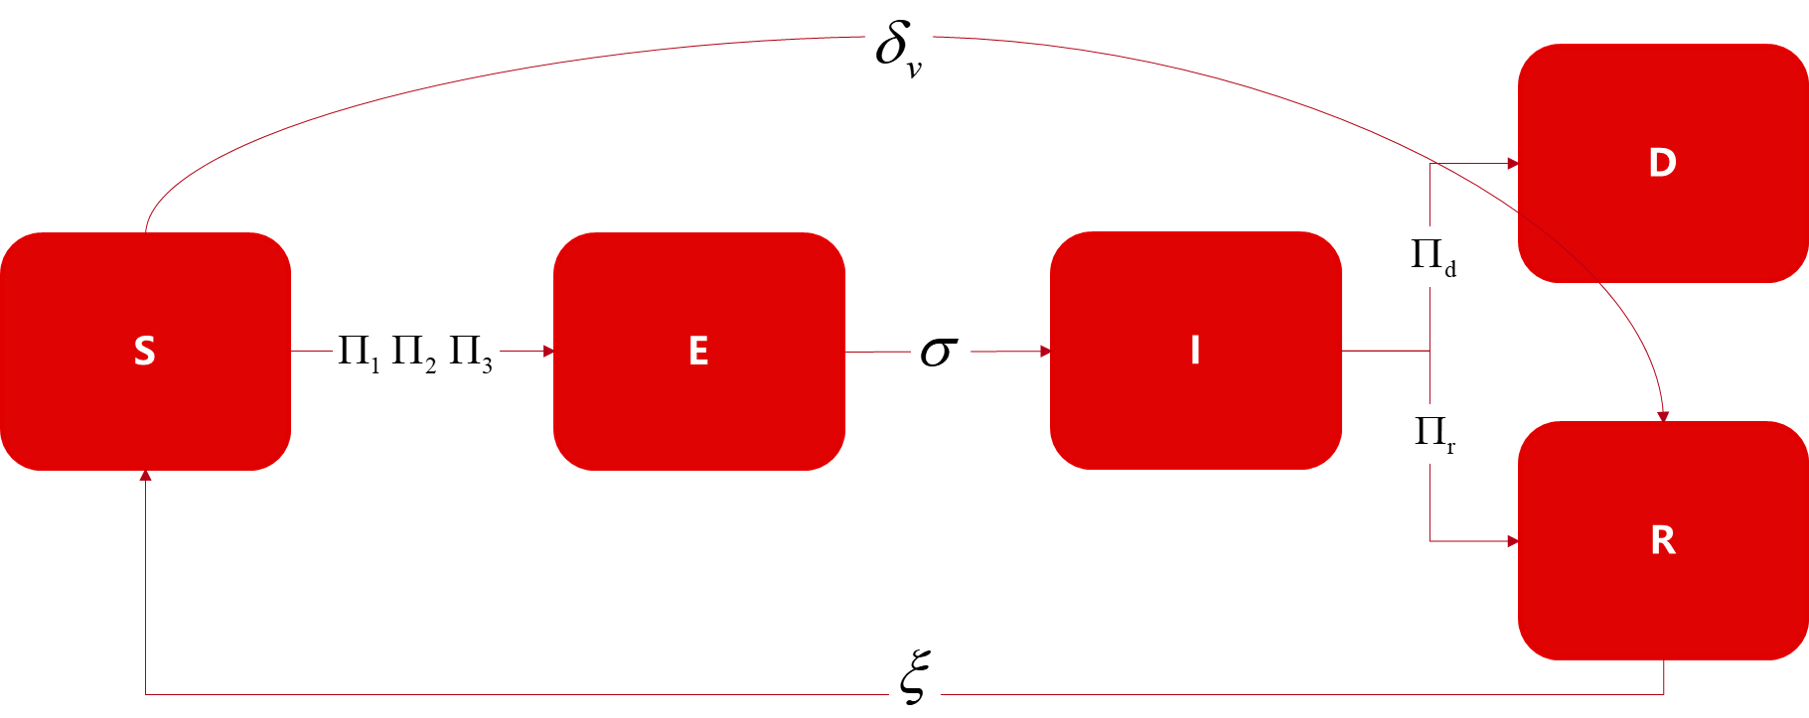
\includegraphics[width=0.8\textwidth]{fig/image057.png}
    \caption{SEIR模型示意图}
    \label{fig:ima29}
\end{figure}

则我们根据$S_t$,$E_t$,$I_t$,$R_t$,$D_t$,$T_t$,$Pop_t$六类人群构建STEIRD模型方程组,描述各类人群相关作用下随时间t变化的发展情况。其动力学示意图如\autoref{fig:ima29}所示。
\begin{equation}\label{seir}
    \left\{
    \begin{array}{ll}
    T_t = \Pi_1(S_t C_{t}^{s})(I_t C_{t}^{i}+E_t C_{t}^{e}) + \Pi_2(S_t N_{t}^{s})(I_t N_{t}^{i}+E_t N_{t}^{e}) + \Pi_3 S_{t}(I_{t}+E_{t}), \\
    S_{t+1}=S_{t} + \xi R_{t} -T_{t} ,   \\  %-\delta_v
    E_{t+1}=E_{t}+T_{t}-\sigma E_t ,  \\  % - \rho_e E_{t}
    I_{t+1}=I_{t}+\sigma E_t- (\Pi_r+\Pi_d)I_{t} ,  \\  % - \rho_i I_{t}
    R_{t+1}=R_{t}+\Pi_r I_t - \xi R_{t} , \\ %+\delta{v}
    D_{t+1}=D_{t}+\Pi_d I_t , \\
    Pop_{t+1}=Pop_{t} - \Pi_d I_t .
    \end{array}
    \right.
\end{equation}

再设$\Delta Y_t= Y_{t+1}-Y_{t}$,其中$Y=S,E,I,R$,则该模型变为:
\begin{align*}
    \Delta S_t=\xi R_{t} -T_{t}, \\
    \Delta E_t=T_{t}-\sigma E_t, \\
    \Delta I_t=\sigma E_t- (\Pi_r+\Pi_d)I_{t}, \\
    \Delta R_t=\Pi_r I_t - \xi R_{t}.
\end{align*}
之后本文使用向量和矩阵来简化表达式,设各类人群的状态、消费及工作时间分别为:$X_t=(S_t,E_t,I_t,R_t)^T$,$C_t=(C_{t}^{s},C_{t}^{e},C_{t}^{i},C_{t}^{r})^T$,$n_t=(n_{t}^{s},n_{t}^{e},n_{t}^{i},n_{t}^{r})^T$,
然后我们设$x=(x_1,x_2,x_3,x_4)^T$,$c=(c_1,c_2,c_3,c_4)^T$,$n=(n_1,n_2,n_3,n_4)^T$,同时定义
\begin{align}
    T(x,c,n)=\Pi_1x_1c_1(x_2c_2+x_3c_3)+\Pi_2x_1n_1(x_2n_2+x_3n_3)+\Pi_3x_1(x_2+x_3).
\end{align}
\begin{align}
    F(x,c,n)=(\xi x_4-T(x,c,n),T(x,c,n)-\sigma x_2, \sigma x_2-(\Pi_r+\Pi_d)x_3,\Pi_r x_3-\xi x_4)^T.
\end{align}
则这个系统可以描述为:
\begin{align}
    \Delta X_t=F(X_t,C_t,n_t).
\end{align}
\subsection{效用模型}
\subsubsection{效用函数}
本文研究的是人的理性行为,在正常时间内选择适当的消费和工作时间来实现自身福利的最大化。设最大化目标函数为:
\begin{align}\label{mubiao}
    U = \sum_{t=0}^{\infty} \beta^t u(c_t,n_t).
\end{align}
在(\ref{mubiao})中,$\beta \in (0,1)$表示折扣系数,$c_t$和$n_t$分别表示消费和工作时间。

为简单起见,我们假设该瞬时效用函数来模拟个人从消费和工作中获得的效用:
\begin{align}
    u(c,n) = lnc - \frac{\theta}{2} n^2.
\end{align}
其中,c是消费,n是工作时间。在这个效用中,第一项衡量的是消费效用,第二项衡量的是工作效用,$\theta$是这两项之间的权重。用$A$表示一个人每小时的平均工资,那么一个工作$n$小时的人的劳动收入为$A*n$,这将是消费的上限,即$n\leq An$。

参数$\theta$不易估算。我们假定当前的消费和工作行为都是最优的,从而将其固定下来。用$n_0$表示病毒传播前单位时间内的全部工作时间。如果一个人按照$n_0$的最优方式工作,那么他的劳动收入为$An_0$。由于效用函数在消费中严格单增,且所有劳动收入都应消费完,因此最优消费$c_0=An_0$,即$\theta = \frac{1}{An_{0}^{2}}$。


% \subsubsection{易感者的效用}
% 设易感者的效用$U_{t}^{s}$为:
% \begin{align}
%     U_{t}^{s} = u(c_{t}^{s},n_{t}^{s}) + \beta[(1-\tau_t)U_{t+1}^{s} + \tau_t U_{t+1}^{i}]
% \end{align}
% 其中$\tau_t$表示易感者被感染的概率,将SEIR模型函数与效用函数联系起来,为:
% \begin{align}\label{yueshu2}
%     \tau_t = \Pi_1 C_{t}^{s}(I_t C_{t}^{i}+E_t C_{t}^{e}) + \Pi_2 N_{t}^{s}(I_t N_{t}^{i}+E_t N_{t}^{e}) + \Pi_3 (I_{t}+E_{t})
% \end{align}

% \subsubsection{感染者的效用}
% 设感染者的效用$U_{t}^{i}$为:
% \begin{align}
%     U_{t}^{i} = u(c_{t}^{i},n_{t}^{i}) + \beta[(1-\Pi_d - \Pi_r)U_{t+1}^{i} + \Pi_r U_{t+1}^{r}]
% \end{align}

% \subsubsection{康复者的效用}
% 设康复者的效用$U_{t}^{e}$为:
% \begin{align}
%     U_{t}^{e} = u(c_{t}^{e},n_{t}^{e}) + \beta[(1-\Pi_d - \Pi_r)U_{t+1}^{e} + \Pi_r U_{t+1}^{r}]
% \end{align}

% \subsubsection{康复者的效用}
% 设感染者的效用$U_{t}^{r}$为:
% \begin{align}
%     U_{t}^{r} = u(c_{t}^{r},n_{t}^{r}) + \beta U_{t+1}^{r}
% \end{align}

\subsubsection{模型约束及控制}
我们设易感者(S)、潜伏者(E)、感染者(I)、康复者(R)单位时间t时效用预算约束为:
\begin{align}\label{con1}
    c_{t}^{s}=&A   n_{t}^{s}, \ \ \ t=0,...,T. \\
    (1+0.9 \mu_t) c_{t}^{e}=&A  n_{t}^{e}, \ \ \ t=0,...,T. \\
    (1+\mu_t) c_{t}^{i}=&A \phi^i n_{t}^{i}, \ \ \ t=0,...,T.  \\
    (1+\mu_t) c_{t}^{r}=&A n_{t}^{r}, \ \ \ t=0,...,T.
\end{align}
其中$\phi^i$表示对易感者工作时间进行管理的控制劳动生产率,设$\phi^i=0.8$,称$\mu_t$为在t时刻的遏制率,其中$\{\mu_t:t\in[0,T]\}$

有了给定的封锁策略$\mu$下每类人群的最佳效用,我们就可以将最优策略制定问题表示为最优控制问题。

\subsection{KKT条件}
\subsubsection{康复者最大效用}
\begin{align}
    J^r(c_.^r,n_.^r;t)=\sum_{t=0}^{T}\beta^t u(c_t^r,n_t^r).
\end{align}
且满足条件$c_t^r \leq  An_t^r$且$n_t^r \leq \frac{1}{1+\mu_t}n_0$。

则在时间t时状态为$X_t$,其遏制率为$\{\mu_t:t\in[0,T]\}$,则最优的$(c_r,n_r)$为:
\begin{align*}
    c_{t}^{r*}=&A n_{t}^{r} \frac{1}{1+\mu_t},\ n_t^{r*}=n_0\frac{1}{1+\mu_t} \ \ \ t=0,...,T.
\end{align*}

针对这种不等式约束优化的内部解和边界解问题,我们可以通过KKT证明其为必要条件:
因为$\frac{\partial J^r(c_.^r,n_.^r;t)}{\partial c_t^r}=\beta^t\frac{1}{c_t^r} >0$,说明其单调递增,则$c_{t}^{r*}=A n_{t}^{r}\ \ \ t=0,...,T.$

设$f(c^r,n^r,\lambda_n^r;t)=J^r(c_.^r,n_.^r;t)+\sum_{t=0}^{T}\lambda_{nt}^r(n_0\frac{1}{1+\mu_t}-n_t^r)$。其中$\lambda_{nt}^r$为对应的$n_0\frac{1}{1+\mu_t}-n_t^r$的拉格朗日乘子。
对拉格朗日函数求导,在$\forall t=0,...,T$上,我们有
\begin{align*}
    \frac{\partial f(c^r*,n^r,\lambda_n^r;t)}{\partial n_t^r}&=0\Rightarrow \\
	\beta^t(-\theta n_t^r+\frac{1}{n_t^r})-\lambda_{nt}^r&=0, \lambda_{nt}^r(n_0\frac{1}{1+\mu_t}-n_t^r)=0, \ \ \lambda_{nt}^r \geq 0 ,
\end{align*}
因为$n_0^2\theta=1$,
\begin{align*}
    \lambda_{nt}^r=\beta^t(-\theta n_t^r+\frac{1}{n_t^r}) \geq \beta^t(-\theta n_0+\frac{1}{n_0})=0.
\end{align*}
其中拉格朗日乘子$\lambda_{nt}^r \geq 0$表明满足对偶可行性,且$\lambda_{nt}^r(n_0\frac{1}{1+\mu_t}-n_t^r)=0$满足互补松弛性,有条件可得$n_0\frac{1}{1+\mu_t}-n_t^r \geq 0$,该条件称之为原始可行性。在这些条件都满足的情况下,则KKT条件成立。

则可得$c_{t}^{r*}=A n_{t}^{r} \frac{1}{1+\mu_t},\ n_t^{r*}=n_0\frac{1}{1+\mu_t} \ \ \ t=0,...,T.$。

同时由于复阳率较低,我们认为康复者对病毒的传播影响非常小,因此康复者的行为不会影响其他人群。
\subsubsection{感染者最大效用}

由上文可知,感染者由于被感染,他们的健康状况通常比其他人更差,则我们通过设定一个常数$\phi$来表示他们的工作效率,易知在$n_t$工作时间内得到的劳动收入为$A*\phi*n$,同时在t时刻的感染者在下一个单位时间内康复的概率为$\Pi_r$,在下一个单位时间内死亡的概率为$\Pi_d$,则$1-\Pi_r-\Pi_d$为留在感染人群中的概率。我们将这些概率设为最大效用中的条件概率。
同时,如果在t时刻康复,之后的效用应为康复者的效用,如果在t时刻死亡,就停止积累效用,因此,得出感染者从0时刻起的累计效用为:
\begin{align}\label{grxy}
    J^i(c_{.}^{i},n_{.}^{i};t)=\sum_{t=0}^{T}\beta^t[(1-\Pi_r-\Pi_d)u(c_t^i,n_t^i)-\Pi_r u(c_t^{r*},n_t^{r*})] .
\end{align}
在\ref{grxy}中,$(c^{r*},n^{r*})$是由康复者累计最优效用决定的。

则在时间t时状态为$X_t$,其遏制率为$\{\mu_t:t\in[0,T]\}$,则最优的$(c_i,n_i)$为:
\begin{align*}
    c_{t}^{i*}=&A \phi n_{t}^{i} \frac{1}{1+\mu_t},\ n_t^{i*}=n_0\frac{1}{1+\mu_t} \ \ \ t=0,...,T.
\end{align*}

以下为通过KKT证明其为必要条件的方法:
因为$\frac{\partial J^i(c_.^i,n_.^i;t)}{\partial c_t^i}=\beta^t (1-\Pi_r-\Pi_d) \frac{1}{c_t^i} >0$,说明其单调递增,则$c_{t}^{i*}=A \phi n_{t}^{i}\ \ \ t=0,...,T.$

设$f(c^i,n^i,\lambda_n^i;t)=J^i(c_.^i,n_.^i;t)+\sum_{t=0}^{T}\lambda_{nt}^i (n_0\frac{1}{1+\mu_t}-n_t^i)$。其中$\lambda_{nt}^i$为对应的$n_0\frac{1}{1+\mu_t}-n_t^i$的拉格朗日乘子。
对拉格朗日函数求导,在$\forall t=0,...,T$上,我们有

\begin{align*}
    \frac{\partial f(c^i*,n^i,\lambda_n^i;t)}{\partial n_t^i}&=0\Rightarrow \beta^t(1-\Pi_r-\Pi_d)(-\theta n_t^i+\frac{1}{n_t^i})-\lambda_{nt}^i=0, \\
    \lambda_{nt}^i&(n_0\frac{1}{1+\mu_t}-n_t^i)=0, \ \ \lambda_{nt}^i \geq 0 ,
\end{align*}
因为$n_0^2\theta=1$,
\begin{align*}
    \lambda_{nt}^i=\beta^t(1-\Pi_r-\Pi_d)(-\theta n_t^i+\frac{1}{n_t^i}) \geq \beta^t(1-\Pi_r-\Pi_d)(-\theta n_0+\frac{1}{n_0})=0.
\end{align*}
其中拉格朗日乘子$\lambda_{nt}^i \geq 0$表明满足对偶可行性,且$\lambda_{nt}^i(n_0\frac{1}{1+\mu_t}-n_t^i)=0$满足互补松弛性,有条件可得$n_0\frac{1}{1+\mu_t}-n_t^i \geq 0$,该条件称之为原始可行性。在这些条件都满足的情况下,则KKT条件成立。

则可得$c_{t}^{i*}=A \phi n_{t}^{i} \frac{1}{1+\mu_t},\ n_t^{i*}=n_0\frac{1}{1+\mu_t} \ \ \ t=0,...,T.$。

同时由于奥密克戎新冠疫情的强烈传播性,感染者的社交行为$(c^i,n^i)$将对易感者的最优决策产生很大影响。

\subsubsection{潜伏者最大效用}

由康复者和感染者的最大效用类比可知,潜伏者的最大效用为:$c_{t}^{e*}=A n_{t}^{i} \frac{1}{1+0.9 \mu_t},\ n_t^{i*}=n_0\frac{1}{1+0.9 \mu_t} \ \ \ t=0,...,T.$。

\subsubsection{易感者最大效用}

根据Eichenbaum\cite{eichenbaum2021macroeconomics}等人所说,为了降低易感人群最优决策目标函数的复杂程度,我们引入感染者的最优价值函数。
假设给定一个被感染前的消费和工作时间组合的时间段为易感者的最优效用,即$(c_t^s,n_t^s)_{t=0,1,...,T}$,则在$t+1$时间将遵循感染后的消费和工作时间,即切换到感染者的最优控制上。因此,得出易感者从0时刻起的累计效用为:
\begin{align}
    J^s(c_{.}^{s},n_{.}^{s},X_t,\mu_.)=u(c_t^s,n_t^s)+\beta \tau_t J^{i*}(t+1,\mu_.)+\beta(1-\tau_t)J^s(c_.^s,n_.^s;t+1,X_{t+1},\mu_.).
\end{align}
其中$\tau_t=\Pi_1 n_0 A \phi I_t \frac{1}{1+\mu_t} c_t^s+\Pi_2 A n_0 I_t \frac{1}{1+\mu_t} n_t^s+\Pi_3 I_t$为在一个时间段t易感者被感染的概率,$J^{i*}(t+1,\mu_.)$为从$t+1$时刻感染者的最优效用函数,
其中$X_{t+1}$为$t+1$时刻的$SEIR$状态,由$t$时刻的$SEIR$状态和各类人群消费和工作的行为$(c_t^s,n_t^s,c_t{i*},n_t^{i*},c_t^{r*},n_t^{r*})$推得。

则我们现在要最大化这个效用函数,即易感者的最优行为:
\begin{equation}
    \begin{aligned}
    \max_{\mu_{.}}&J^s(c_.^s,n_.^s;\mu_{.},t,X_t), \\
    s.t.& \ \ \ c_t^s \leq A n_t^s,\ \ , n_t^s \leq n_0 \frac{1}{1+\mu_t}, \ \ \forall t \in [0,T].
    \end{aligned}
\end{equation}

在这里我们需要证明在t时刻的状态$X_t$及控制率$\{\mu_t:t\in[0,T]\}$下,易感者的消费和工作时间最优解为:
\begin{align}
    c_t^{s*}=A n_t^{s*}, \ \ \ t=0,...,T.
\end{align}

证明如下:

我们设一个价值函数为$V(t,X_t)=J^s(c_.^{s*},n_.^{s*};t,X_t,\mu_.)$,由动态规划原理的最优子结构我们可知:
\begin{align*}
    V(t,X_t)&=\max_{c_t^s \leq A n_t^s,n_t^s \leq \frac{1}{1+\mu_t}} [u(c_t^s,n_t^s)+\beta \tau_t J^{i*}(t+1,\mu_.)+\beta(1-\tau_t)V(t+1,X_{t+1})] \\
    &=u(c_t^{s*},n_t^{s*})+\beta \tau_t^{*}J^{i*}(t+1,\mu_.)+\beta(1-\tau_t^*)V(t+1,X_{t+1}^*).
\end{align*}
其中$\tau_t^*$为易感者被感染的概率,$X_{t+1}^*$为$t+1$时刻的$SEIR$状态。

使用反证法,假设$c_t^{s*} < An_t^{s*}$,由于$\tau_t$关于$c^s$和$n^s$单调递增,我们能找到一个值$m \in (c_t^{s*},An_t^{s*})$,设另一个控制为$c_t^s=m$和$n_t^s=\frac{m}{A}$,则$\tau_t=\tau_t^*$,即$X_{t+1}=X_t^*$,但是因为$c_t^s > c_t^{s*}$和$n_t^s<n_t^{s*}$,
我们有$u(c_t^s,n_t^s)>u(c_t^{s*},n_t^{s*})$,与$(c^{s*},n^{s*})$为动态规划方程的最优解相矛盾,则$c_t^{s*}=An_t^{s*}$。

\subsection{最优控制策略}
政府可以通过多种方式减少人们的接触,比如关闭餐馆和娱乐活动场所;让人们居家办公等,与Farhi\cite{farhi2012dealing}等人对资本管制的处理相似。通过给定控制$\mu_.$的各类人群的最优行为,将该问题转化为最优控制问题,我们定义$J^0(L_.;t,X_t)$为不同人的效用的加权平均值作为最优控制函数。
我们设从$t=0$时刻开始,$S_0=s$,$E_0=e$,$I_0=i$,$R_0=r$,状态为$X_0=(S_0,E_0,I_0,R_0)^T$,则我们得到这个最优控制问题为:
\begin{align}\label{yuan}
    \max_{\mu_{.}}J^0(\mu_{.},t,X_t)&=\sum_{t=0}^{T} \beta^t[S_t u(c_t^{s*},n_t^{s*})+E_t u(c_t^{e*},n_t^{e*})+I_t u(c_t^{i*},n_t^{i*})+R_t u(c_t^{r*},n_t^{r*})].
\end{align}
其中$(c_t^{a*},n_t^{a*}) \ \ (a=s,e,i,r)$为由KKT条件求得的各类人群的最优消费和最优工作时间。

在$J^0$中,我们忽视了死亡者造成的负效用,因为其效用较小,可以忽略不计,但是不仅要关注死亡者对造成的经济损失,还要考虑到死亡带给社会精神层面的冲击,由于传染病导致的死亡对家庭和社会有很大的负面影响,政府部门不能忽略死亡者造成的负效用,则在目标函数中引入死亡惩罚系数$\alpha$来表明对社会产生的强烈影响。设为:
\begin{equation}\label{xin}
	\begin{aligned}
		J^{\alpha}(\mu_{.},t,X_t)=&\sum_{t=0}^{T} \beta^t[S_t u(c_t^{s*},n_t^{s*})+E_t u(c_t^{e*},n_t^{e*})+I_t u(c_t^{i*},n_t^{i*}) \\
		&+R_t u(c_t^{r*},n_t^{r*})-\alpha D_t u(c_t^{r*},n_t^{r*})].
	\end{aligned}
\end{equation}
%\begin{align}\label{xin}
%    J^{\alpha}(\mu_{.},t,X_t)=\sum_{t=0}^{T} \beta^t[S_t u(c_t^{s*},n_t^{s*})+E_t u(c_t^{e*},n_t^{e*})+I_t u(c_t^{i*},n_t^{i*}) 
%    +R_t u(c_t^{r*},n_t^{r*})-\alpha D_t u(c_t^{r*},n_t^{r*})].
%\end{align}
在$J^{\alpha}$中,我们用康复者的最优效用来表示死亡者对社会的影响大小,$\alpha$的取值视作政府对死亡严重程度的评估。当$\alpha=0$,函数\ref{xin}变为函数\ref{yuan}。

则我们需要求解的目标函数为:
\begin{equation}
    \begin{aligned}
    \max_{\mu_{.}}&J^{\alpha}(\mu_{.},t,X_t), \\
    s.t. \ \ \ &\mu_t\in[0,1], \ \ \forall t \in [0,T].
    \end{aligned}
\end{equation}




% \begin{equation}
%     \begin{aligned}
%         \max_{L.} J^0(L.;t,X_t)=&\sum_{t=t_0}^{T}\beta^{t-t_0}[S_t u(c_{t}^{s^*},n_{t}^{s^*})+I_t u(c_{t}^{i^*},n_{t}^{i^*})+R_t u(c_{t}^{r^*},n_{t}^{r^*})]\\
%         s.t. \ L_t &\in[0,1] \ \forall t \in[0,T].    
%     \end{aligned}        
% \end{equation}

\section{扩展SEIR宏观模型求解}

\subsection{fmincon算法}
参考Eichenbaum\cite{eichenbaum2021macroeconomics}等人的文章可知这个最优控制模型结构良好,康复者、潜伏者和感染者的最优决策是可以忽略掉的,可以只求解易感人群的最优决策问题。
由于存在约束,我们很难得到一个确定的解,我们将每个时间点的最优控制视为带有消费和工作时间控制政策两个约束条件的静态优化,通过求解KKT条件来获得解。将最优控制$(c^{s^*},n^{s^*})$作为封锁策略L的函数,通过MATLAB工具箱fmincon的基于梯度的内点法,对每个时间点进行求解。

\subsection{参数估计}
在本文的扩展SEIR宏观模型中,我们对一个单位时间的要求比较宽泛,可以视作一个不同人群从奥密克戎爆发开始到结束转移变化的趋势,不用把每个点作为一天或一周。
对与死亡率$\Pi_d$和治愈率$\Pi_r$本文参考Eichenbaum\cite{eichenbaum2021macroeconomics}等人使用韩国卫生和福利局在2022年奥密克戎的数据,同时我们也参考了Salje\cite{salje2020estimating}等人感染人群恢复或死亡的概率。且Ferguson\cite{ferguson2006strategies}等人认为对于流行病感染传播,$30\%$的传播发生在家庭,$33\%$发生在社区,$37\%$发生在学校和公众场合;为了拟合这些估计到我们的参数中,参考美国劳工统计局$(ATUS)$统计数据来估算消费和工作时间占用外出时间的百分比,
得到$\Pi_1=1.244887\times 10^{-6}$,$\Pi_2=1.0336 \times 10^{-4}$,$\Pi_3=0.01759$,$\Pi_r=0.78656$,$\Pi_d=0.00033$。

另外我们参考Fu\cite{fu2022optimal}的文章,根据ONS的数据统计了近几年来全职员工每周平均的工作时间为36.9,则我们设$n_0=36.9$,由等式$n_0^2*\theta=1$,我们设$\theta=0.0073$。

我们也考虑到了病毒会导致感染者的工作效率降低,设定为$\phi_i=0.8$。同时根据潜伏者在病毒未爆发前无法监测出来,监管措施和个人防护会有所疏忽,所以我们设定潜伏者的遏制率要低于对感染者的遏制率,设为$0.9\mu_t$。

为了简化流行病学模型,我们将起始人口设为1,所有的人数都可以看作是初始时间$t=0$时总人口的百分比。此外,我们将单位时间段设为一天,避免记录数据的延迟,可以显示流行病的变化。表\ref{chart}列出了数值实验中常用的参数和数值。
\begin{table}[h]
    \centering
    \caption{模型参数}\label{chart}
    \begin{tabular}{c|c|c}
        \hline
        变量 & 含义 & 值 \\
        \hline
        $\pi_1$ & 消费对感染率的贡献 & $1.244887 \times 10^{-6}$ \\
        $\pi_2$ & 工作对感染率的贡献 & $1.0336 \times 10^{-4}$\\
        $\pi_3$ & 其他活动对感染率的贡献 & $0.01759$ \\
        $\pi_r$ & 感染者恢复的概率 & $0.78656$ \\
        $\pi_d$ & 感染者死亡的概率 & $0.00033$ \\
        $n_0$ & 满负荷工作时间 & $36.9$ \\
        $\theta$ & 消费函数和工作函数的效用权重 & $\frac{1}{(36.9)^2}$ \\
        $\xi$ & 感染者复阳的概率 & $0.05$ \\
        $\sigma$ & 潜伏人群转化为感染人群的概率 & $0.33333$ \\
        $\phi^i$ & 对感染者工作时间进行管理的控制劳动生产率 & $0.8$ \\
        $\alpha$ & 死亡惩罚系数 & $0; \ 100; \ 200; \ 400$ \\
        $\delta_v$ & 每个时期发现疫苗的概率 & $\frac{1}{52}$ \\
		\hline
    \end{tabular}
    \end{table}



\vspace{35em}
\subsection{数值结果}
在本节中,我们介绍由以上参数设置下的实验结果。通过实验来分析最优控制策略,包括提前结束遏制策略、较晚开始封锁策略及一些灵活的遏制策略等。我们参考Fu Yuting\cite{fu2022optimal}等人设定初始数据为$(S,E,I,R)=(0.9990,0.0008,0.0002,0)$。

\subsubsection{最优控制策略}
如\autoref{fig:ima1}、\autoref{fig:ima2}所示,如果没有控制策略,即$\mu_t=0$,则感染者和潜伏者会在第40个时间点达到最高峰,根据数值计算显示,大概有$90\%$的人口会被感染,而在我们的最优控制政策中,在第40个时间点的感染人数接近为0,并在之后的第100个时间点也没有超过$2\%$;如\autoref{fig:ima5}所示,在没有控制的情况下死亡比例为$0.9475*10^(-3)$,在有最优控制策略的情况下,死亡比例为$0.8450*10^(-5)$,将死亡人数降低了$84.229\%$,维护了很多人的生命安全。
如\autoref{fig:ima6}所示,在开始阶段不带有控制策略的总消耗量为7.59,带有控制的总消耗量为4.67,但是在第60个时间之后,不带有控制策略的总消耗量增速开始降低,而最优控制策略的总消耗量保持稳定增长,从而最优控制策略反超,在第90个时间点,不带控制的总消耗量为16.214,最优控制的总消耗量为27.862,远远高于不带控制策略的消费。针对最优控制策略没有导致经济进一步衰退的原因,我们猜测感染人数降低,易感人数被感染的概率降低,保证了易感染人群的工作时间以及他们的生活状态,减少了很多非必要的损失。

如\autoref{fig:ima7}所示,最佳控制率从$50\%$左右开始,在0\~{}30这个时间段内,控制率曲线升高的速率先增加再降低,在第30个时间点左右达到峰值为$87.82\%$,之后开始缓慢下降,直到第65个时间点降低到$74.67\%$,之后在缓慢上升,总体来说,控制率的曲线一个动态变化的过程,根据每个时间点的感染人数动态调整控制率,比较符合现实中的宏观调控。同时我们的模型是在130个时间点之内,其结果不能包含整个病毒传播过程。

% 插入2*3个图片
\begin{figure}[htbp]
	\centering
	\begin{minipage}{0.49\linewidth}
		\centering
		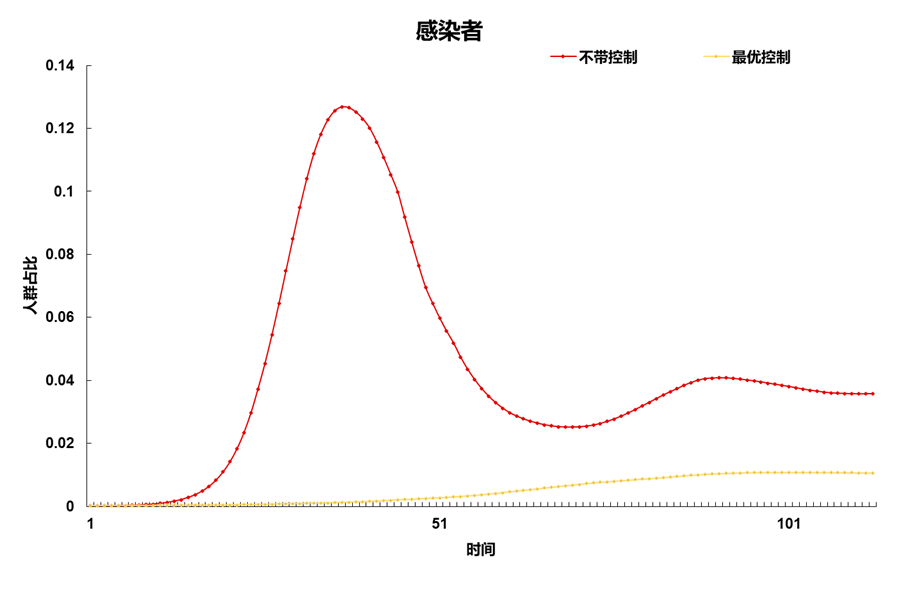
\includegraphics[width=0.9\linewidth]{fig/image002.png}
		\caption{最优控制下的感染者}
		\label{fig:ima1}%文中引用该图片代号
	\end{minipage}
	\begin{minipage}{0.49\linewidth}
		\centering
		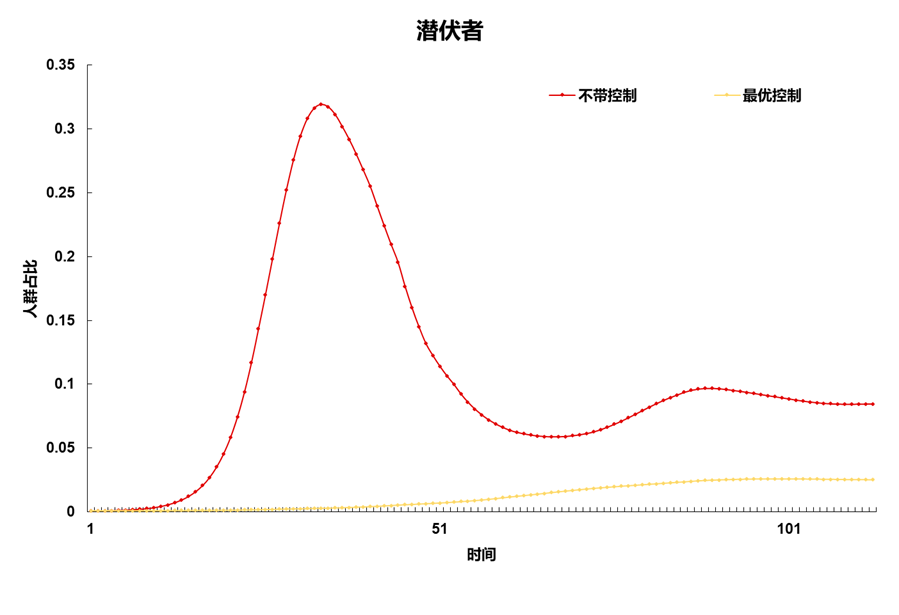
\includegraphics[width=0.9\linewidth]{fig/image010.png}
		\caption{最优控制下的潜伏者}
		\label{fig:ima2}%文中引用该图片代号
	\end{minipage}
	%\qquad
	%让图片换行,
	
	\begin{minipage}{0.49\linewidth}
		\centering
		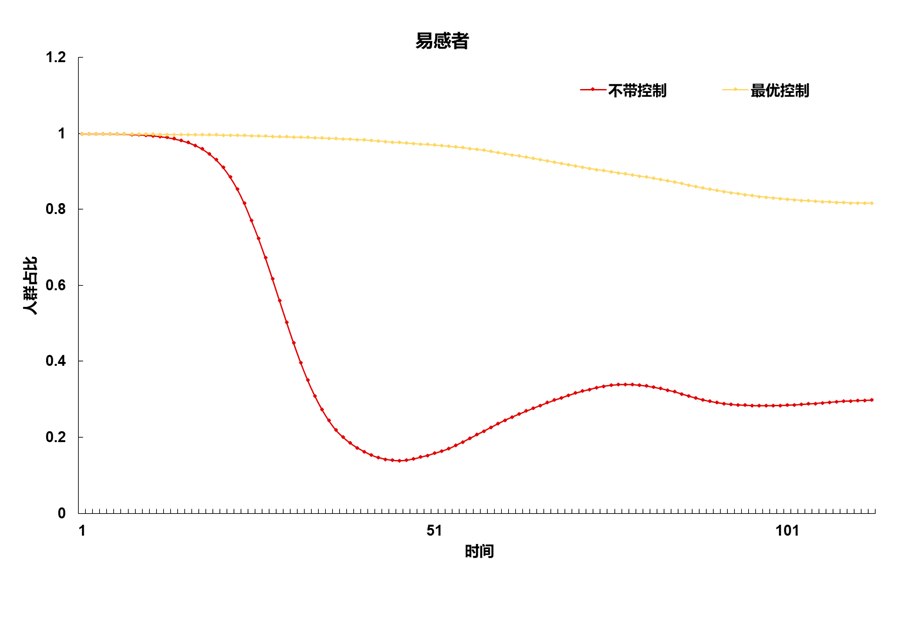
\includegraphics[width=0.9\linewidth]{fig/image008.png}
		\caption{最优控制下的易感者}
		\label{fig:ima3}%文中引用该图片代号
	\end{minipage}
	\begin{minipage}{0.49\linewidth}
		\centering
		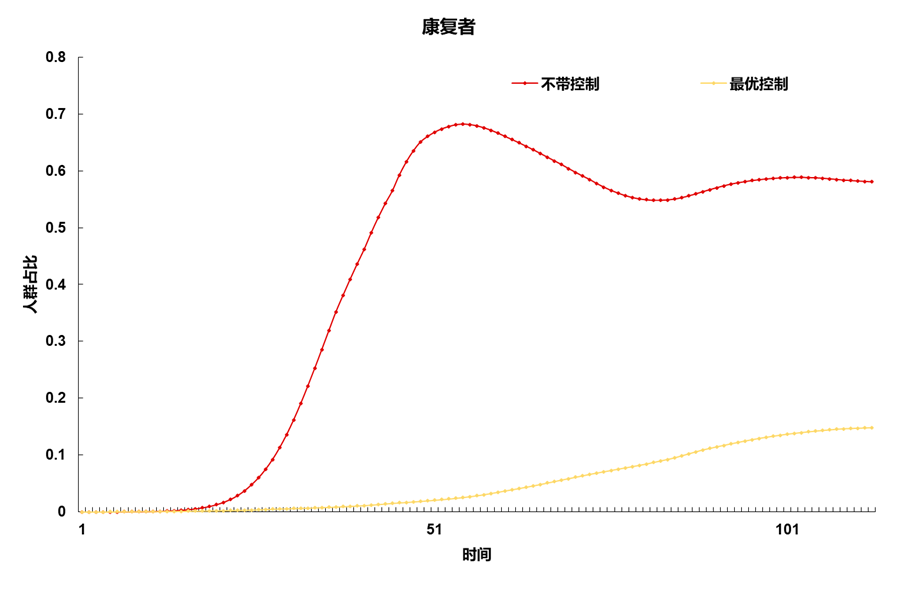
\includegraphics[width=0.9\linewidth]{fig/image012.png}
		\caption{最优控制下的康复者}
		\label{fig:ima4}%文中引用该图片代号
	\end{minipage}

    \begin{minipage}{0.49\linewidth}
		\centering
		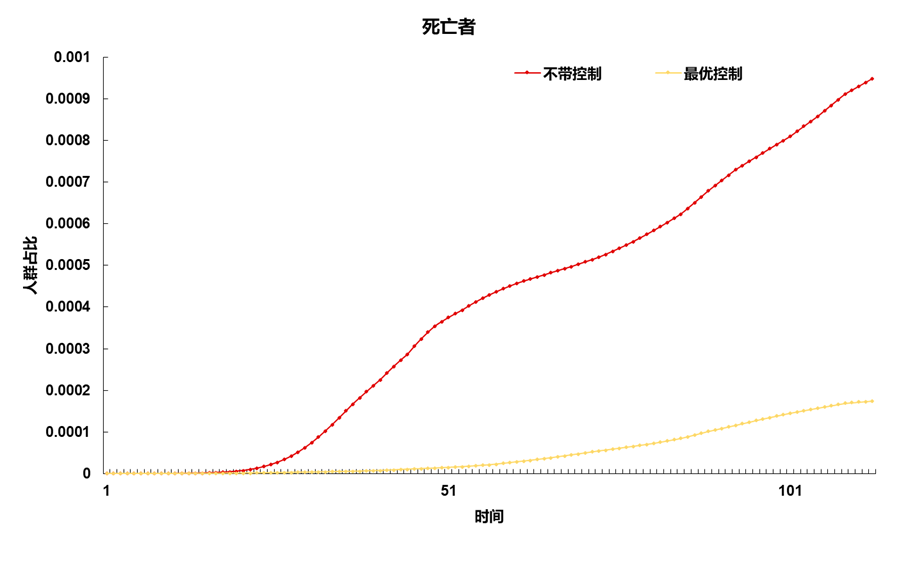
\includegraphics[width=0.9\linewidth]{fig/image014.png}
		\caption{最优控制下的死亡者}
		\label{fig:ima5}%文中引用该图片代号
	\end{minipage}
	\begin{minipage}{0.49\linewidth}
		\centering
		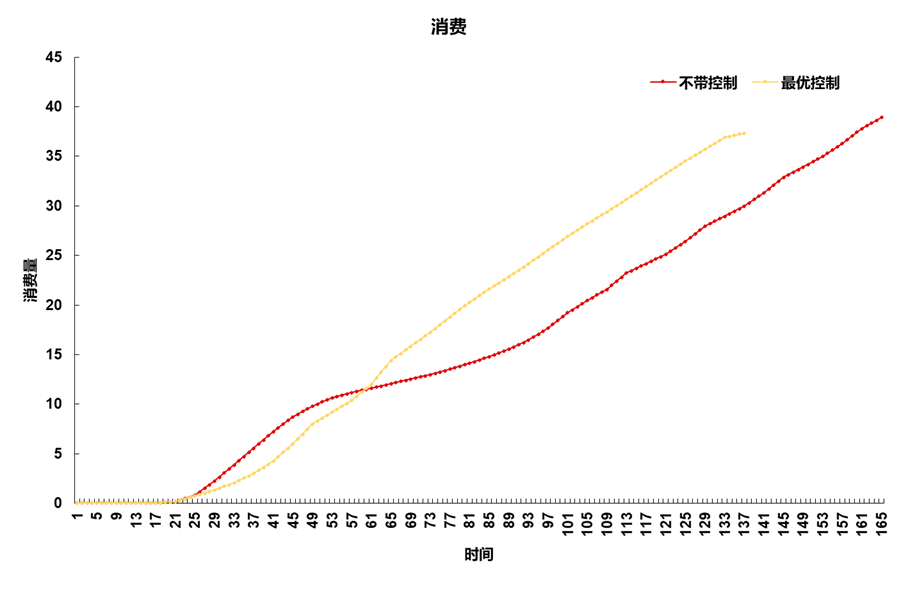
\includegraphics[width=0.9\linewidth]{fig/image004.png}
		\caption{最优控制下的消费}
		\label{fig:ima6}%文中引用该图片代号
	\end{minipage}

	\begin{minipage}{0.49\linewidth}
		\centering
		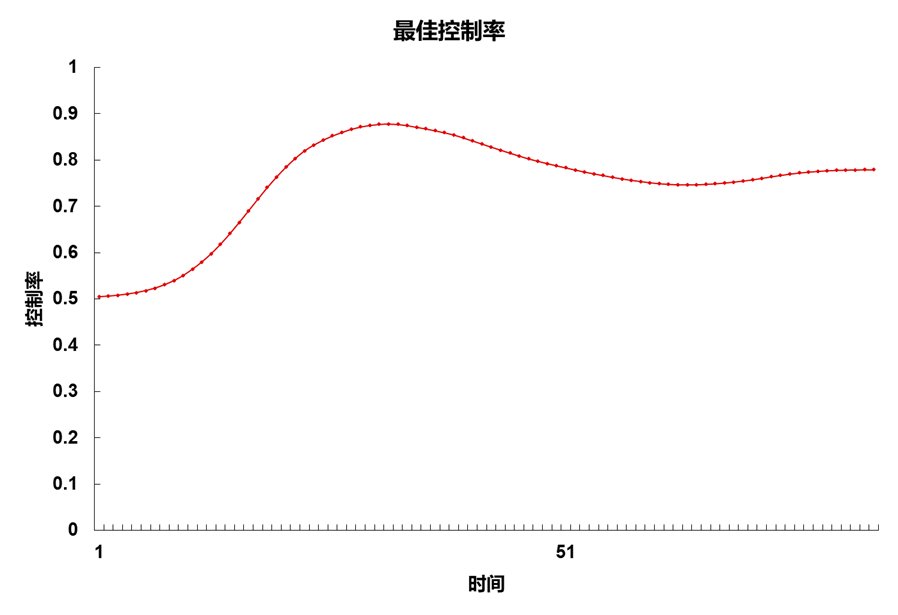
\includegraphics[width=0.9\linewidth]{fig/image006.png}
		\caption{最优控制率}
		\label{fig:ima7}%文中引用该图片代号
	\end{minipage}
\end{figure}
% 最优控制率

\vspace{135em }
\subsubsection{带有死亡惩罚系数的最优控制策略}
在本节中,考虑死亡的严重程度会影响最优控制策略,所以我们引入死亡惩罚系数$\alpha$,设其为0、100、200和400,即策略制定者认为一个人的死亡相当于0、100、200、400个康复者的效用。当$\alpha=0$时,与原最优控制模型相同。
当我们增加死亡惩罚系数的值时,如\autoref{fig:ima8}所示,避免了感染者的大幅上升,死亡惩罚系数为0、100、200、400的感染者的峰值分别为$82.67\%$,$78.62\%$,$77.26\%$,$74.39\%$。表明死亡对社会上人们的情绪调动是有一定影响的,较低的死亡者和感染者会减轻策略制定者的压力,从而改善最优控制策略。
同时由\autoref{fig:ima9}可知,当我们假如死亡惩罚系数后,与原来的最优控制策略的消费比较有所降低,当我们设定惩罚系数为100,200,400时,其对应的消费分别降低了$1.6\%$,$13.5\%$,$31.7\%$,说明死亡惩罚系数增加会带动人群的恐慌情绪,会比在最优控制下的消费还要低,所以,当我们考虑更高的死亡成本时会作出更加保守的控制决策,以更大的经济衰退为代价降低死亡率。
% 死亡惩罚 
\begin{figure}[htbp]
	\centering
	\begin{minipage}{0.49\linewidth}
		\centering
		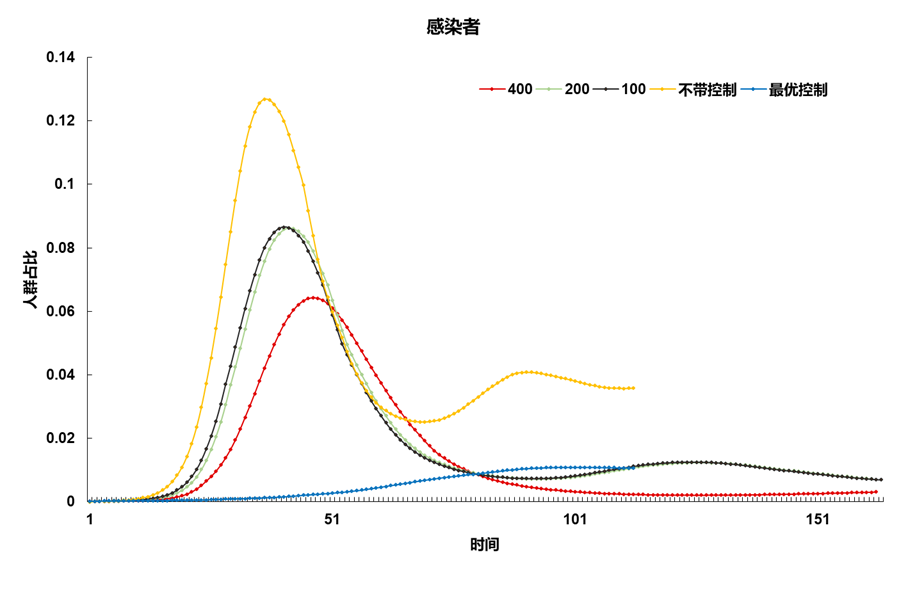
\includegraphics[width=0.9\linewidth]{fig/image016.png}
		\caption{死亡惩罚下的感染者}
		\label{fig:ima8}%文中引用该图片代号
	\end{minipage}
	\begin{minipage}{0.49\linewidth}
		\centering
		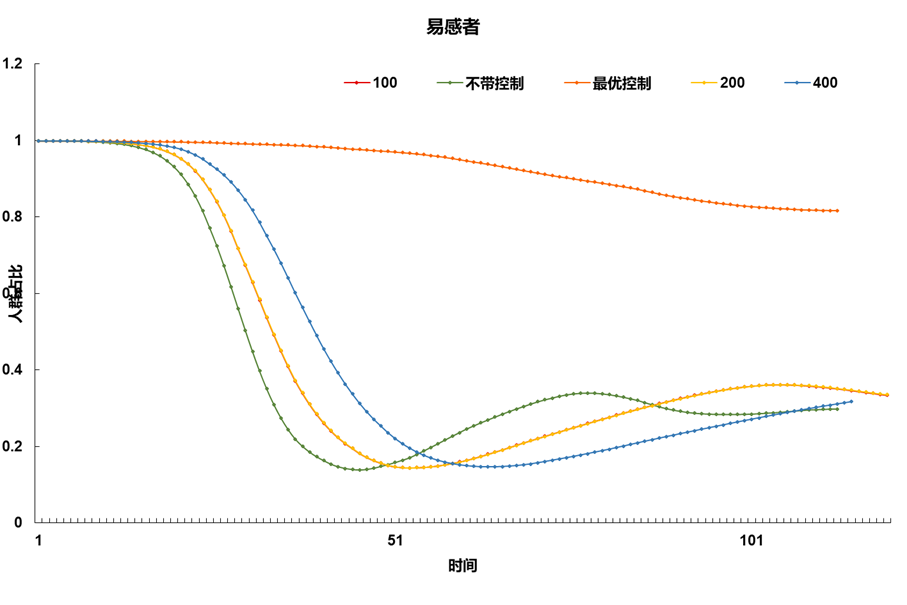
\includegraphics[width=0.9\linewidth]{fig/image018.png}
		\caption{死亡惩罚下的易感者}
		\label{fig:ima9}%文中引用该图片代号
	\end{minipage}
	%\qquad
	%让图片换行,
	
	\begin{minipage}{0.49\linewidth}
		\centering
		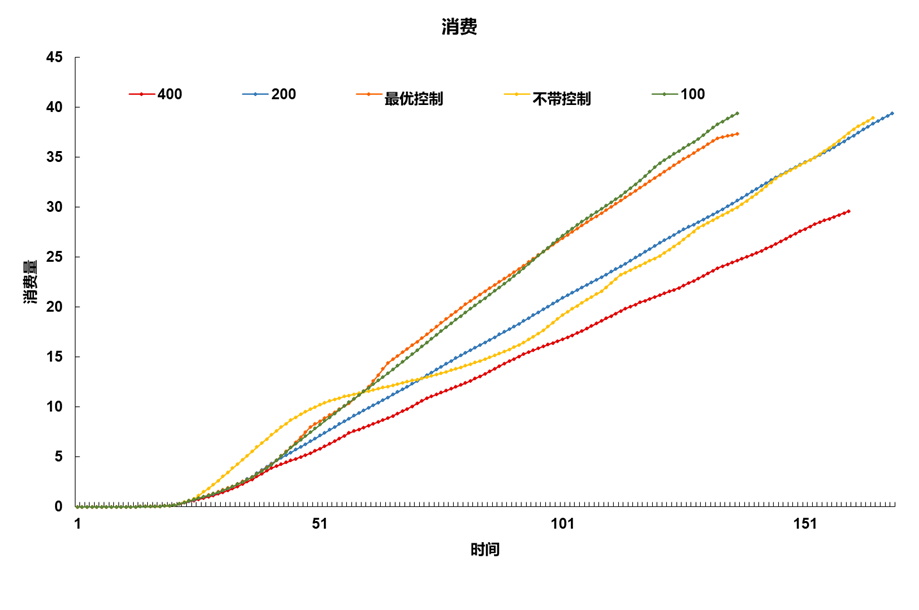
\includegraphics[width=0.9\linewidth]{fig/image020.png}
		\caption{死亡惩罚下的消费}
		\label{fig:ima10}%文中引用该图片代号
	\end{minipage}

\end{figure}

\subsubsection{提前结束控制的策略}
在现实中,政府由于舆论压力和经济压力可能会提前结束控制策略恢复正常的经济水平。在本节中,我们讨论提前退出控制后人群及消费的变化。在这里我们设在第61个时间点解除控制策略。
如\autoref{fig:ima16}可知,封锁后的经济相比最优控制期间没有明显增长,而且如\autoref{fig:ima11}和\autoref{fig:ima12}所示,会导致感染者及潜伏者数量的迅速反弹,在峰值处比最优控制策略下增加了69倍多,同时,在感染者爆发的高峰期总消费量相较于最优控制降低了4.68。

由此可知策略制定者不能过早结束控制策略,不仅没有导致消费的增加、经济活力的提高,还会导致感染群体进一步增加,死亡者数量提高。
\begin{figure}[htbp]
	\centering
	\begin{minipage}{0.49\linewidth}
		\centering
		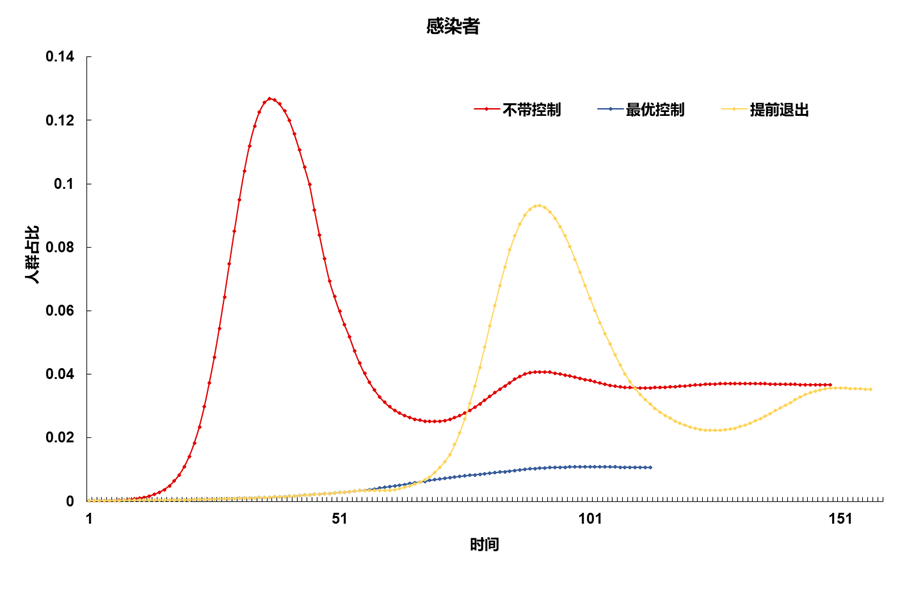
\includegraphics[width=0.9\linewidth]{fig/image024.png}
		\caption{提前结束控制的感染者}
		\label{fig:ima11}%文中引用该图片代号
	\end{minipage}
	\begin{minipage}{0.49\linewidth}
		\centering
		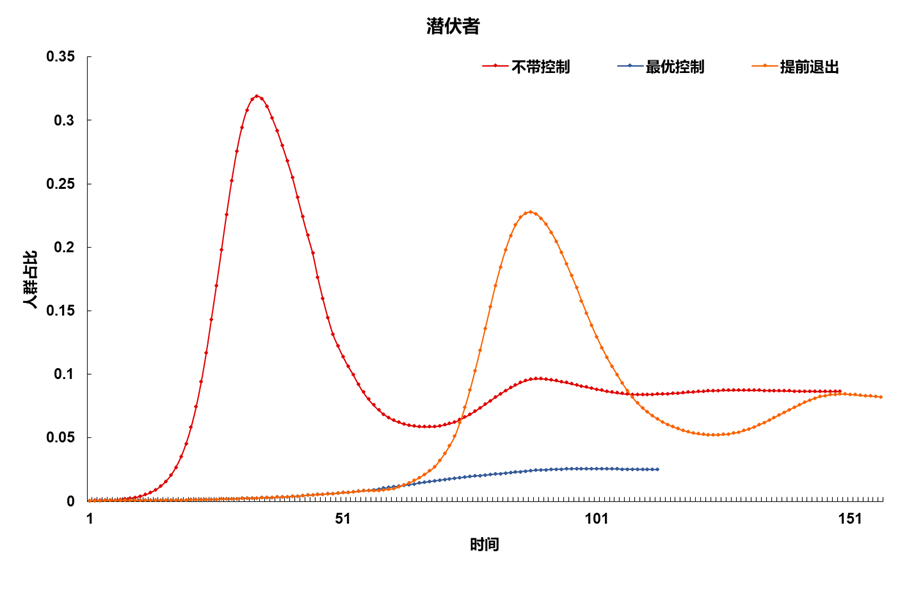
\includegraphics[width=0.9\linewidth]{fig/image032.png}
		\caption{提前结束控制的潜伏者}
		\label{fig:ima12}%文中引用该图片代号
	\end{minipage}
	%\qquad
	%让图片换行,
	
	\begin{minipage}{0.49\linewidth}
		\centering
		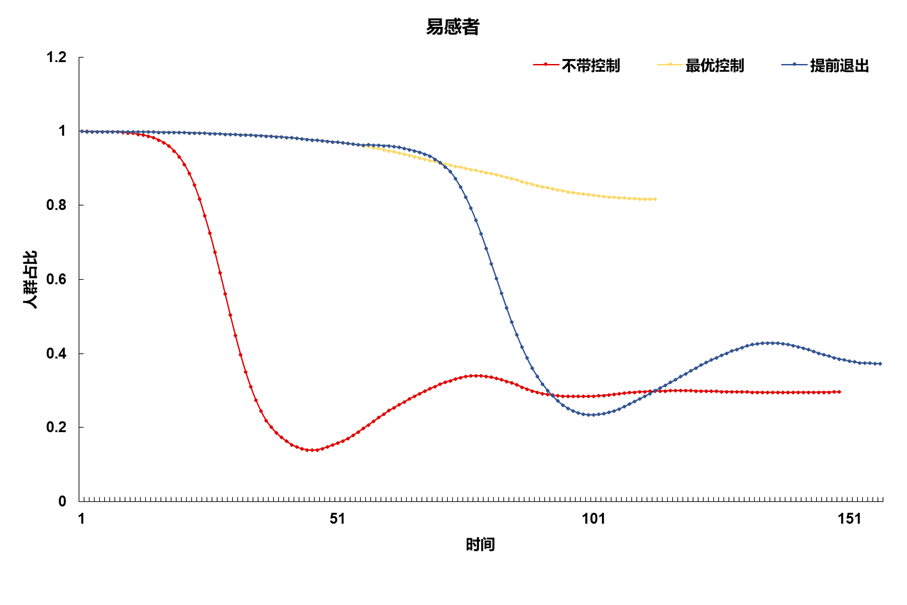
\includegraphics[width=0.9\linewidth]{fig/image028.png}
		\caption{提前结束控制的易感者}
		\label{fig:ima13}%文中引用该图片代号
	\end{minipage}
	\begin{minipage}{0.49\linewidth}
		\centering
		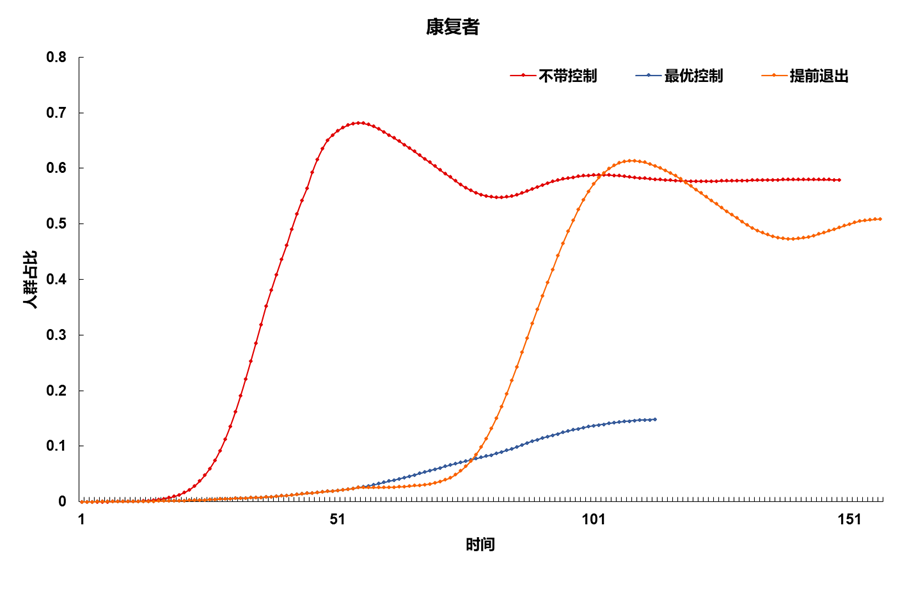
\includegraphics[width=0.9\linewidth]{fig/image026.png}
		\caption{提前结束控制的康复者}
		\label{fig:ima14}%文中引用该图片代号
	\end{minipage}

    \begin{minipage}{0.49\linewidth}
		\centering
		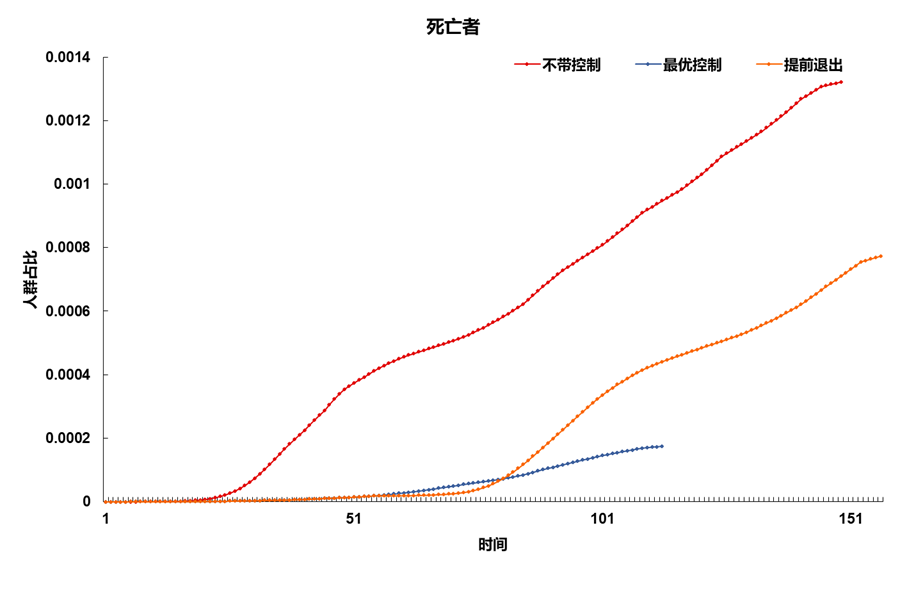
\includegraphics[width=0.9\linewidth]{fig/image030.png}
		\caption{提前结束控制的死亡者}
		\label{fig:ima15}%文中引用该图片代号
	\end{minipage}
	\begin{minipage}{0.49\linewidth}
		\centering
		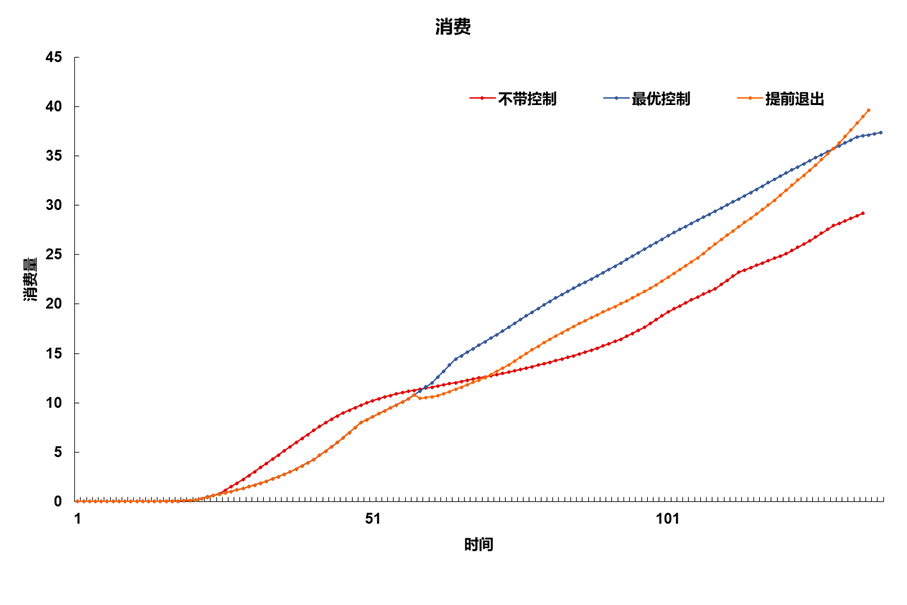
\includegraphics[width=0.9\linewidth]{fig/image022.png}
		\caption{提前结束控制的消费}
		\label{fig:ima16}%文中引用该图片代号
	\end{minipage}
\end{figure}

\subsubsection{较晚开始控制策略}
在这节中,我们讨论在疫情初期可能存在认知不完全、信息差以及管理部门协调不到位这些因素,导致了控制策略较晚开始。
如\autoref{fig:ima21}所示,我们在第38个时间点开始控制策略,与从第1个时间点开始的最优控制策略相比,死亡人数没有得到很好的控制,在其峰值处的死亡者数量为在第一个时间点开始控制策略的死亡人数的101倍。
如\autoref{fig:ima22}所示,当我们在第38个时间点开始控制时,其消费量先是低于不带控制的消费量,最高差值为3.74,之后在第78个时间开始反超。表明在控制之后,虽然开始阶段会带来经济损失,但是长期来看封锁策略能保证稳定的消费水平。
同时尽管较晚开始控制策略保证了感染人群不会进一步扩散、经济水平不会快速衰退,但是消费量始终小于最初的最优控制策略,平均相差5.497个水平。

根据所示图信息,控制策略越早实施越好,虽然初期会带来更低的经济效应,但保证了未来的消费水平不会进一步衰退。
\begin{figure}[htbp]
	\centering
	\begin{minipage}{0.49\linewidth}
		\centering
		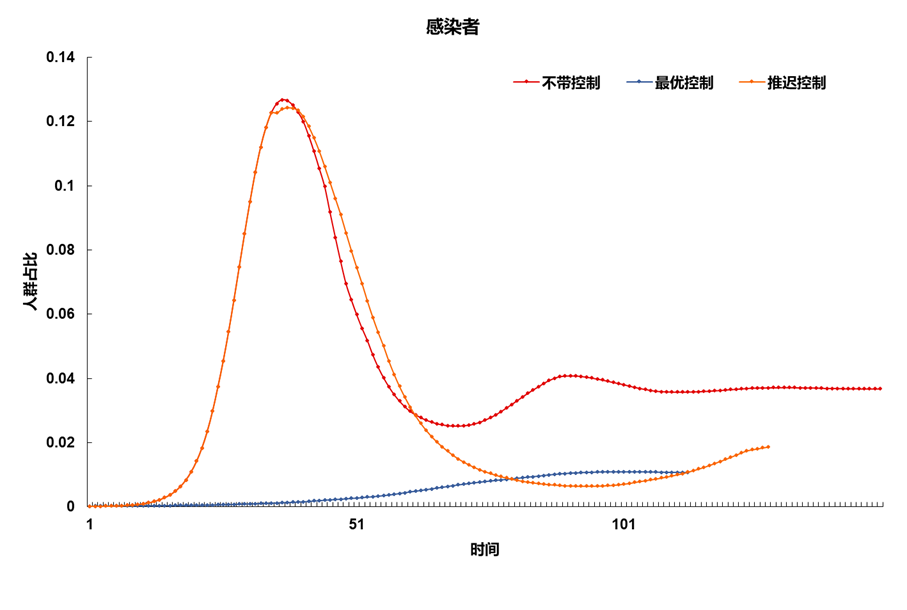
\includegraphics[width=0.9\linewidth]{fig/image036.png}
		\caption{较晚开始控制的感染者}
		\label{fig:ima17}%文中引用该图片代号
	\end{minipage}
	\begin{minipage}{0.49\linewidth}
		\centering
		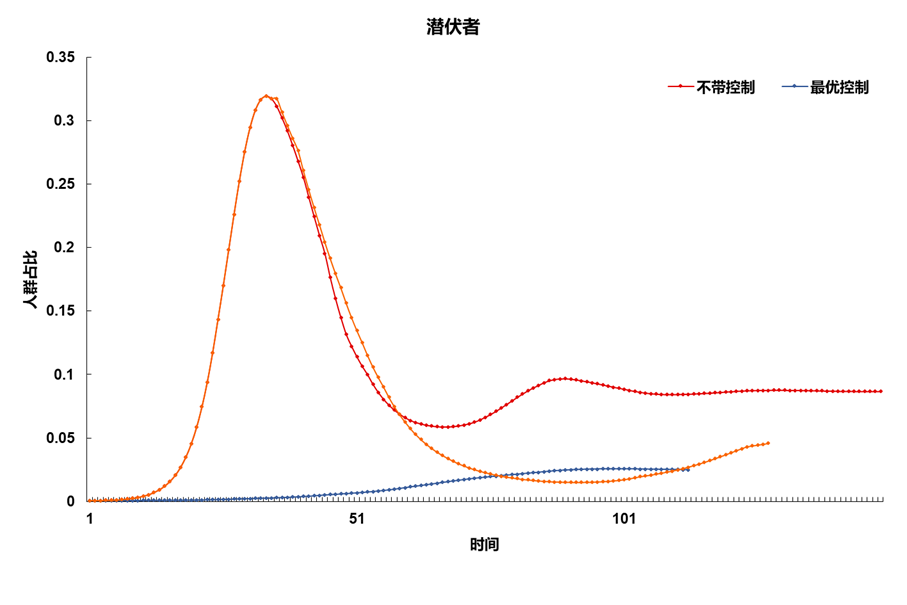
\includegraphics[width=0.9\linewidth]{fig/image040.png}
		\caption{较晚开始控制的潜伏者}
		\label{fig:ima18}%文中引用该图片代号
	\end{minipage}
	%\qquad
	%让图片换行,
	
	\begin{minipage}{0.49\linewidth}
		\centering
		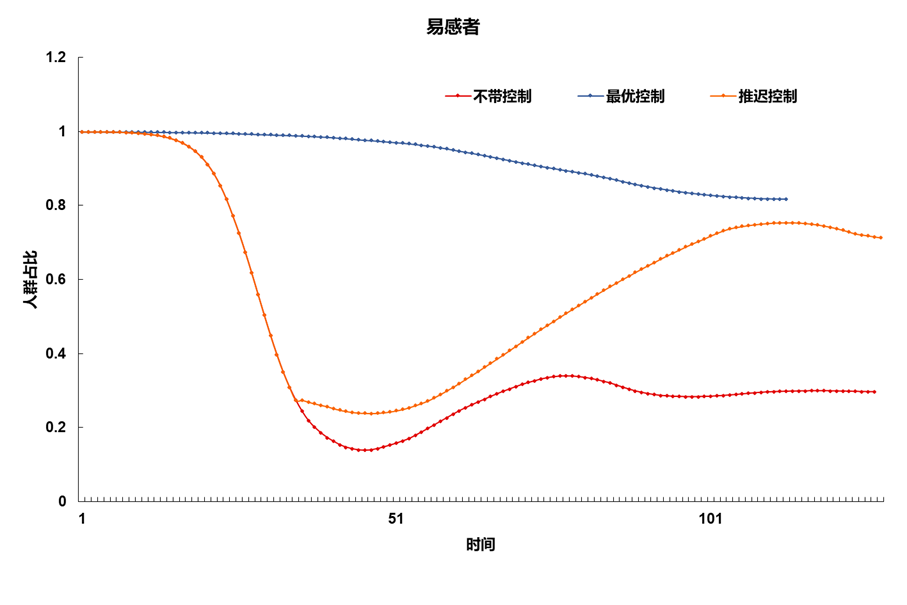
\includegraphics[width=0.9\linewidth]{fig/image038.png}
		\caption{较晚开始控制的易感者}
		\label{fig:ima19}%文中引用该图片代号
	\end{minipage}
	\begin{minipage}{0.49\linewidth}
		\centering
		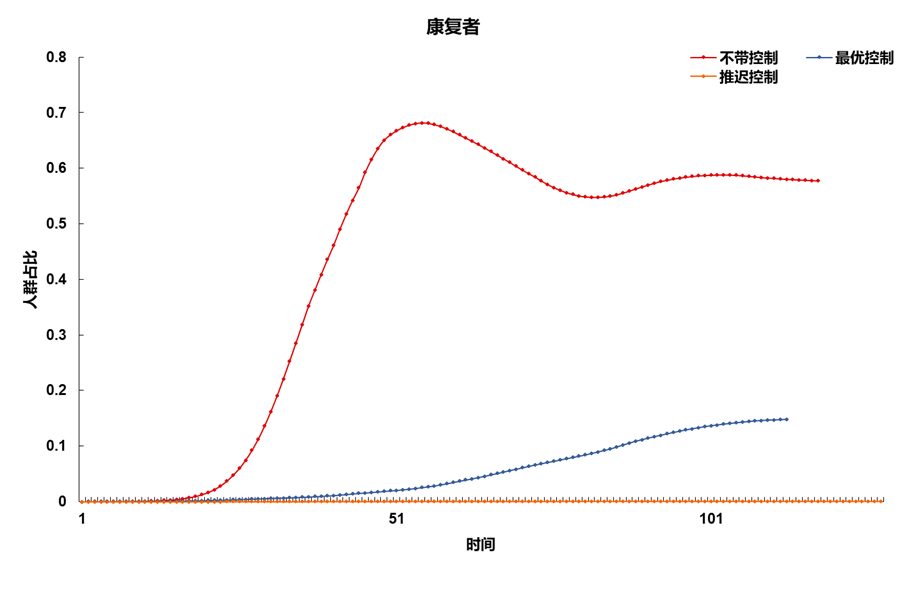
\includegraphics[width=0.9\linewidth]{fig/image042.png}
		\caption{较晚开始控制的康复者}
		\label{fig:ima20}%文中引用该图片代号
	\end{minipage}

    \begin{minipage}{0.49\linewidth}
		\centering
		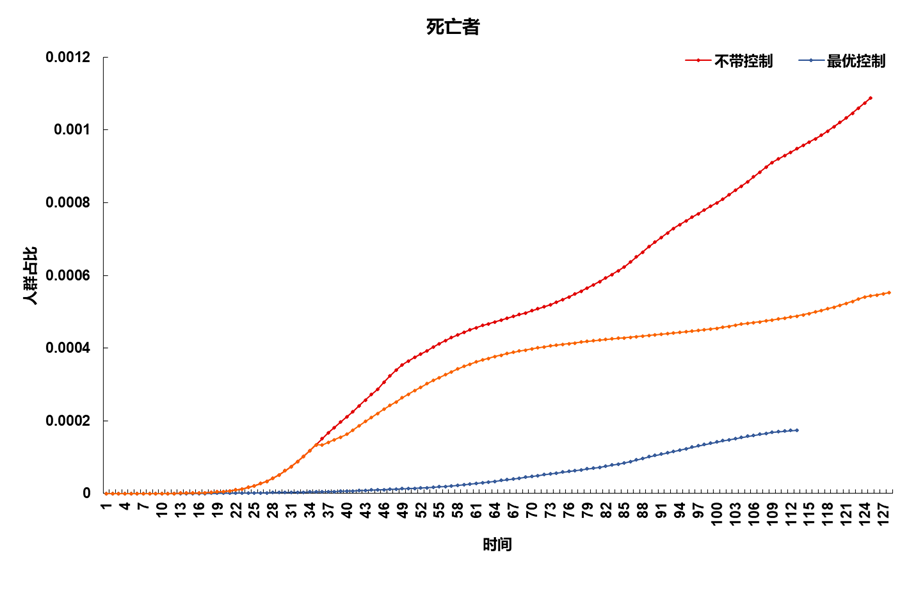
\includegraphics[width=0.9\linewidth]{fig/image044.png}
		\caption{较晚开始控制的死亡者}
		\label{fig:ima21}%文中引用该图片代号
	\end{minipage}
	\begin{minipage}{0.49\linewidth}
		\centering
		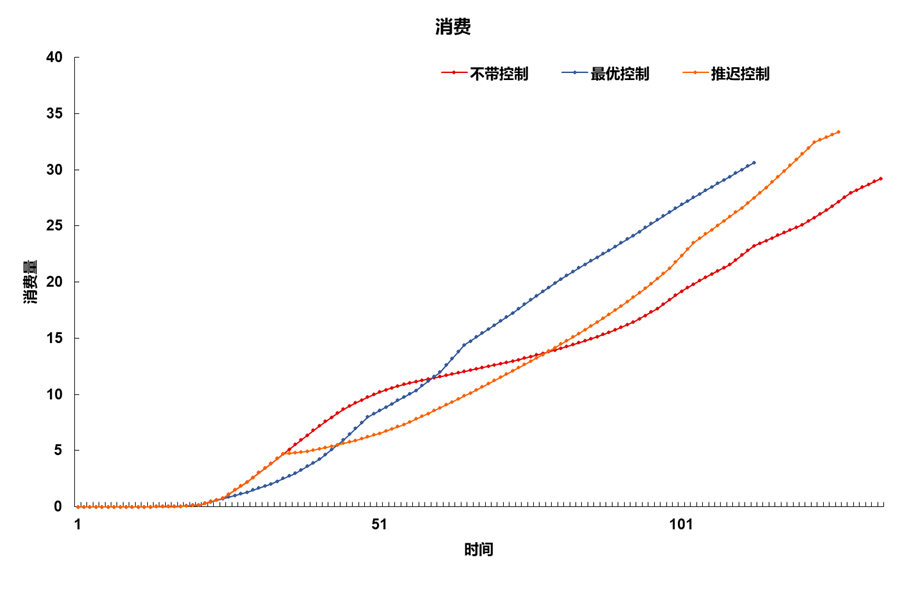
\includegraphics[width=0.9\linewidth]{fig/image034.png}
		\caption{较晚开始控制的消费}
		\label{fig:ima22}%文中引用该图片代号
	\end{minipage}
\end{figure}

\subsubsection{疫苗接种}
疫苗接种是预防流行性病毒的有效方法。在本节中,我们将疫苗纳入SEIR宏观模型,假设每个时期发现疫苗的概率为$\delta_v$,则在每一个时间段,有一定数量的易感人群接种疫苗后可以预防奥密克戎病毒,视作康复者,同时由政府承担疫苗研发和投放的花费。则易感人群的目标函数变为:
\begin{align*}
    J^s(c_{.}^{s},n_{.}^{s},X_t,\mu_.)=&u(c_t^s,n_t^s)+\beta (1-\frac{\delta_v}{S_t}) \tau_t J^{i*}(t+1,\mu_.)+ \\
	&\beta (1-\frac{\delta_v}{S_t}) (1-\tau_t)J^s(c_.^s,n_.^s;t+1,X_{t+1},\mu_.) + \beta \frac{\delta_v}{S_t}J^{r*}(t+1,\mu_.).
\end{align*}

设政府对疫苗的花费为p,则这个最优控制问题变为:
\begin{align}
    \max_{\mu_{.}}J^0(\mu_{.},t,X_t)&=\sum_{t=0}^{T} \beta^t[S_t u(c_t^{s*},n_t^{s*})+E_t u(c_t^{e*},n_t^{e*})+I_t u(c_t^{i*},n_t^{i*})+R_t u(c_t^{r*},n_t^{r*})-p \delta_v].
\end{align}
我们参考Fu\cite{fu2022optimal}对$\delta_v$的估计,设$\delta_v=\frac{1}{52}$。由\autoref{fig:ima23}和\autoref{fig:ima27}可知,与未接种疫苗相比,接种疫苗可以彻底结束疫情,减少死亡人数,同时由\autoref{fig:ima28}可知,接种疫苗后人群的消费强度更高,缓解了经济衰退的严重程度。

\begin{figure}[htbp]
	\centering
	\begin{minipage}{0.49\linewidth}
		\centering
		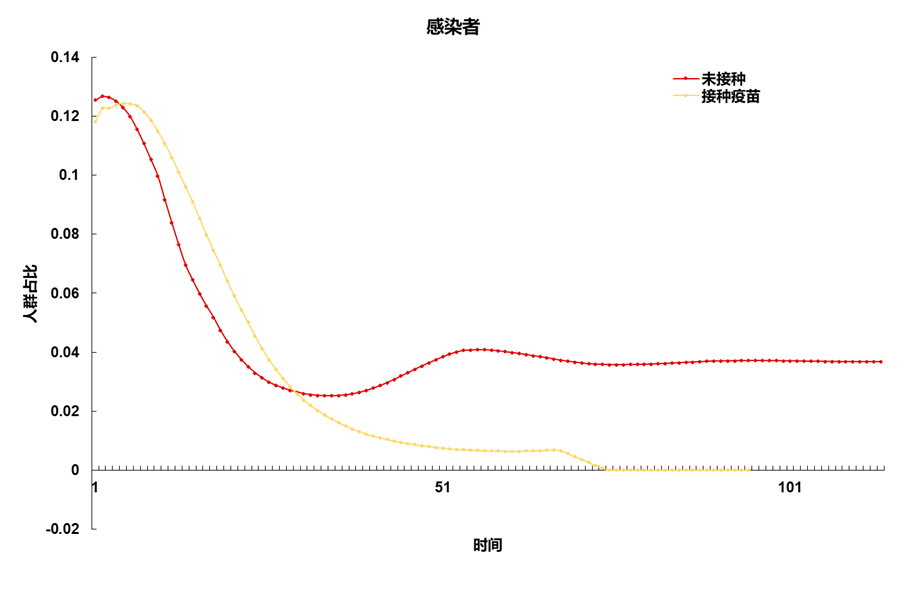
\includegraphics[width=0.9\linewidth]{fig/image055.png}
		\caption{接种疫苗的感染者}
		\label{fig:ima23}%文中引用该图片代号
	\end{minipage}
	\begin{minipage}{0.49\linewidth}
		\centering
		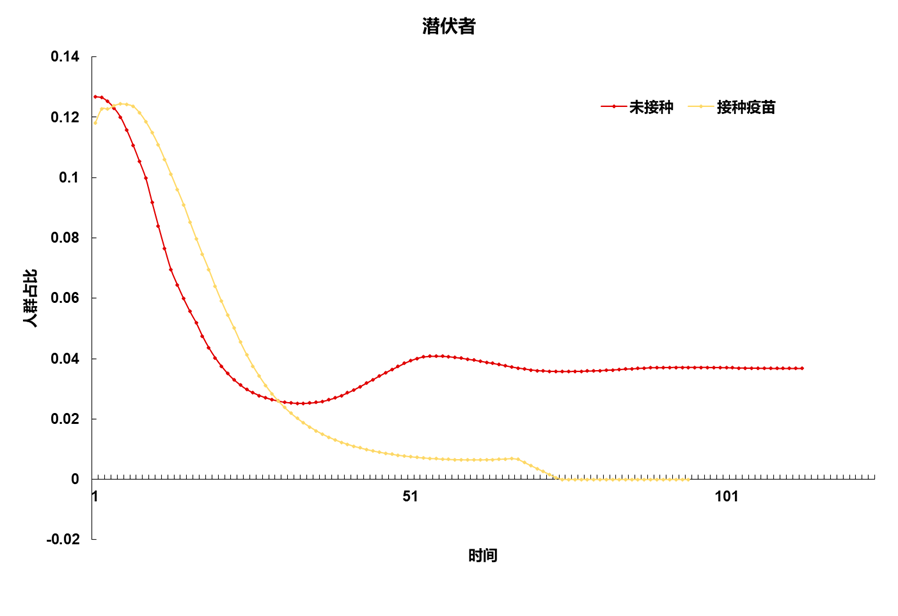
\includegraphics[width=0.9\linewidth]{fig/image049.png}
		\caption{接种疫苗的潜伏者}
		\label{fig:ima24}%文中引用该图片代号
	\end{minipage}
	%\qquad
	%让图片换行,
	
	\begin{minipage}{0.49\linewidth}
		\centering
		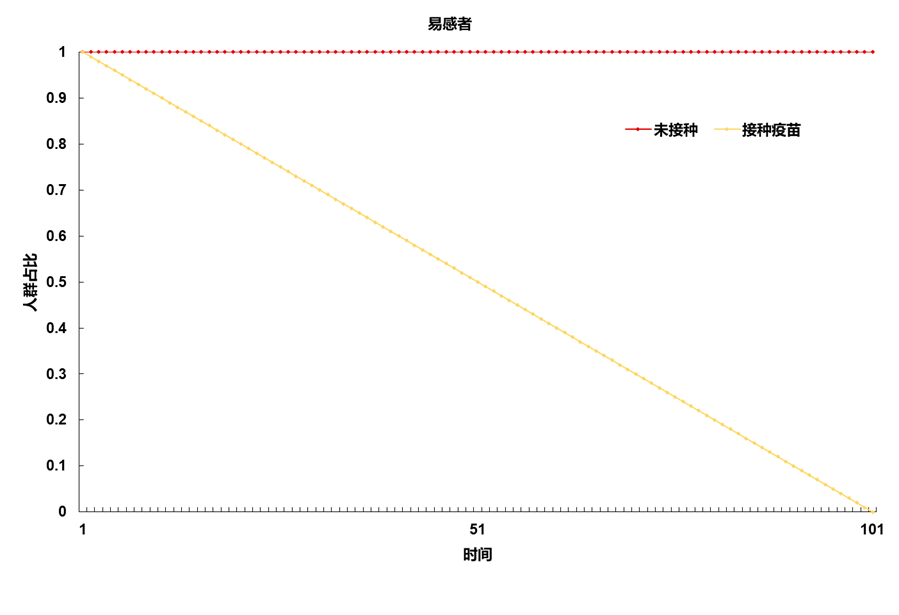
\includegraphics[width=0.9\linewidth]{fig/image045.png}
		\caption{接种疫苗的易感者}
		\label{fig:ima25}%文中引用该图片代号
	\end{minipage}
	\begin{minipage}{0.49\linewidth}
		\centering
		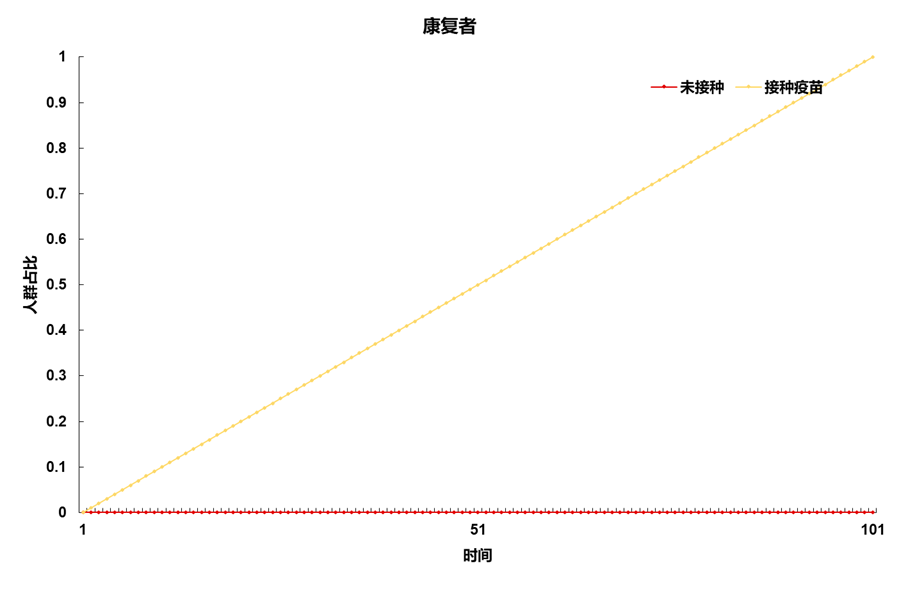
\includegraphics[width=0.9\linewidth]{fig/image047.png}
		\caption{接种疫苗的康复者}
		\label{fig:ima26}%文中引用该图片代号
	\end{minipage}

    \begin{minipage}{0.49\linewidth}
		\centering
		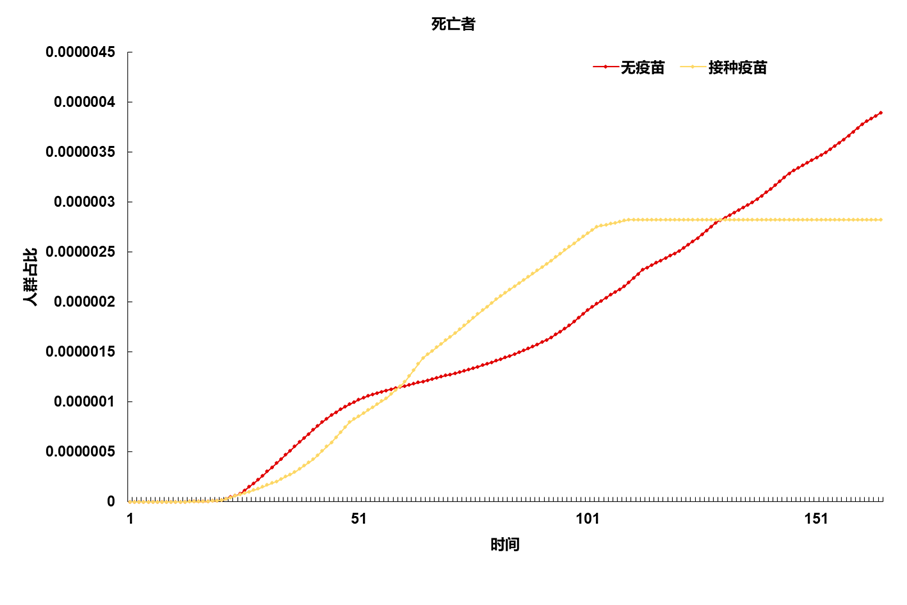
\includegraphics[width=0.9\linewidth]{fig/image051.png}
		\caption{接种疫苗的死亡者}
		\label{fig:ima27}%文中引用该图片代号
	\end{minipage}
	\begin{minipage}{0.49\linewidth}
		\centering
		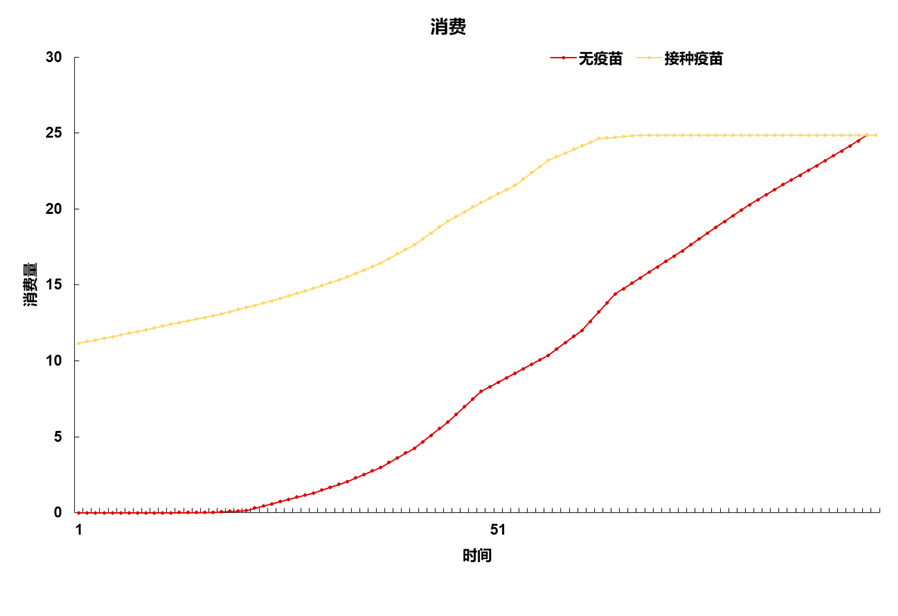
\includegraphics[width=0.9\linewidth]{fig/image053.png}
		\caption{接种疫苗下的消费}
		\label{fig:ima28}%文中引用该图片代号
	\end{minipage}
\end{figure}
\vspace{100em}